\documentclass{informatics-report}

\graphicspath{{figures/}}

% ------------------------------------------------------------
% Metadata
% ------------------------------------------------------------
\newcommand{\ProjectTitle}{Distributed Mutual Exclusion Explorer}
\newcommand{\ProjectSubtitle}{Interactive Tools for Learning Distributed Systems Concepts (Variant 3)}
\newcommand{\StudentName}{Lei Ding}
\newcommand{\StudentID}{K21029011}
\newcommand{\ProgrammeName}{BSc Computer Science}
\newcommand{\SupervisorName}{Angelos Georgoulas}
\newcommand{\DepartmentName}{Department of Informatics, King's College London}

\begin{document}

% ------------------------------------------------------------
% Title page
% ------------------------------------------------------------
\begin{titlepage}
\centering
\vspace*{2.2cm}

{\color{deepblue}\bfseries\LARGE \ProjectTitle\par}
\vspace{0.6cm}
{\Large \ProjectSubtitle\par}

\vspace{2.0cm}

{\large \textbf{Author:} \StudentName\par}
\vspace{0.2cm}
{\large \textbf{Student ID:} \StudentID\par}
\vspace{0.2cm}
{\large \textbf{Programme:} \ProgrammeName\par}

\vspace{1.0cm}

{\large \textbf{Supervisor:} \SupervisorName\par}
\vspace{0.2cm}
{\large \DepartmentName\par}

\vfill

{\large \today\par}
\end{titlepage}

% ------------------------------------------------------------
% Front matter
% ------------------------------------------------------------
\pagenumbering{roman}

\chapter*{Originality Avowal}
\addcontentsline{toc}{chapter}{Originality Avowal}
This report is submitted as part of the requirements for the Final Year Individual Project.
It is the result of the author's own work except where explicitly indicated in the text.
All sources are acknowledged by appropriate references.
This report has not been submitted for any other assessment at this or any other institution.

\chapter*{Abstract}
\addcontentsline{toc}{chapter}{Abstract}
Distributed mutual exclusion is a foundational distributed systems problem, yet its behaviour is difficult to learn from static descriptions because correctness depends on concurrency, ordering, and failure assumptions. This project delivers a browser-based interactive teaching tool that visualises distributed mutual exclusion using two representative approaches: a token-based Token Ring model and a teaching-oriented Ricart--Agrawala (RA) prototype. The tool supports step-by-step execution, scripted demonstrations, fault injection (token loss, crash/recover, and message loss in RA), and evidence export (state JSON, trace TXT, preview PNG) for reproducible evaluation. Correctness is evaluated primarily via the safety property (mutual exclusion), while fault scenarios are used to illustrate the separation between safety and liveness. Testing combines a manual evidence-driven test plan with dependency-free automated smoke tests executed in continuous integration. The resulting artefact provides an accessible environment for exploring distributed coordination and for producing traceable evaluation evidence.

\chapter*{Acknowledgements}
\addcontentsline{toc}{chapter}{Acknowledgements}
The author would like to thank the project supervisor for guidance and feedback throughout the project.

\tableofcontents
\clearpage
\listoffigures
\clearpage
\listoftables
\clearpage

\pagenumbering{arabic}

% ------------------------------------------------------------
% Chapters
% ------------------------------------------------------------
\IfFileExists{Chapters/01_introduction.tex}{\chapter{Introduction}
\label{ch:introduction}

\section{Motivation}
Distributed systems underpin modern computing, but their behaviour is often difficult to understand from static material because correctness depends on concurrency, message ordering, and assumptions about failures \cite{tanenbaum2017distributed,coulouris2011distributed,lynch1996distributed}. Mutual exclusion is a classic example: a set of distributed processes must coordinate access to a shared critical section without relying on shared memory or a global clock.

Learners commonly struggle to connect algorithm descriptions to concrete executions. This challenge becomes more severe when faults are introduced, since safety properties may remain intact even when progress is lost. Such distinctions are difficult to communicate through static diagrams alone. This motivates the development of an interactive teaching tool that makes state, causality, and fault consequences directly observable.

\section{Project Aim and Objectives}
The aim of this project is to develop an interactive educational artefact for visualising distributed mutual exclusion and its behaviour under faults and recovery conditions.

The specific objectives are:
\begin{itemize}
  \item implement a technically correct simulation that preserves the safety invariant of mutual exclusion,
  \item provide step-by-step execution with an explanatory trace,
  \item support representative token-based and message-based algorithms,
  \item support fault injection and recovery to illustrate safety vs liveness trade-offs,
  \item provide reproducible evidence export,
  \item and evaluate the artefact in terms of correctness, usability, and reproducibility.
\end{itemize}

\section{Scope}
The delivered system focuses on two representative approaches:
\begin{itemize}
  \item \textbf{Token Ring}, a token-based mechanism that provides an intuitive model of exclusivity.
  \item \textbf{Ricart--Agrawala (RA)}, a message-based algorithm using Lamport-style timestamps \cite{ricart1981optimal,lamport1978time}.
\end{itemize}

The system is teaching-oriented rather than production-oriented. The network model is intentionally simplified to support controlled observation and reproducibility. Message loss in RA is used to demonstrate that liveness can fail while safety is preserved; retransmission and failure detectors are not implemented.

\section{Contributions}
The main contributions of the project are:
\begin{itemize}
  \item a browser-based, dependency-free Distributed Mutual Exclusion Explorer,
  \item support for both Token Ring and an RA teaching-oriented prototype,
  \item explicit fault injection and recovery mechanisms,
  \item scripted demos for deterministic replay,
  \item an evidence export pipeline (state JSON, trace TXT, preview PNG),
  \item and a reproducible testing and evidence framework built around a freeze baseline.
\end{itemize}

\section{Report Structure}
Chapter~\ref{ch:background} reviews distributed mutual exclusion, logical time, fault assumptions, and educational visualisation literature.
Chapter~\ref{ch:design} presents the specification and design of the artefact.
Chapter~\ref{ch:implementation} describes implementation details.
Chapter~\ref{ch:testing} covers testing strategy and execution.
Chapter~\ref{ch:evaluation} evaluates correctness, usability, and reproducibility.
Chapter~\ref{ch:professional} discusses professional issues.
Chapter~\ref{ch:conclusion} concludes the report and outlines future work.}{}
\IfFileExists{Chapters/02_background.tex}{\chapter{Background and Related Work}
\label{ch:background}

\section{Distributed Mutual Exclusion}
Distributed mutual exclusion requires a set of processes to coordinate access to a critical section using message passing rather than shared memory. Two correctness dimensions are central:
\begin{itemize}
  \item \textbf{Safety:} at most one process may enter the critical section at any time.
  \item \textbf{Liveness:} requesting processes should eventually make progress under suitable assumptions.
\end{itemize}
This safety--liveness distinction is fundamental in distributed systems and forms the theoretical basis of this project \cite{lynch1996distributed,attiya2004distributed,tel2000introduction}.

Mutual exclusion algorithms can be grouped into message-based, token-based, and hierarchical or tree-based families. Each family makes different assumptions and offers different teaching affordances. This project intentionally implements one token-based approach and one message-based approach in order to provide contrast rather than breadth.

\section{Message-Based and Token-Based Approaches}
Message-based algorithms coordinate access through explicit REQUEST/REPLY exchanges. Ricart--Agrawala (RA) is one of the classical examples, requiring each requesting process to receive permission from all peers before entering the critical section \cite{ricart1981optimal}. Maekawa's algorithm reduces the number of messages through quorums, but introduces additional conceptual complexity in explaining quorum intersections and deadlock handling \cite{maekawa1985sqrt}.

Token-based algorithms instead rely on possession of a unique token. This makes the safety mechanism conceptually simple: a process may enter the critical section only when it holds the token. Suzuki--Kasami is a well-known token-based algorithm for distributed mutual exclusion \cite{suzuki1985distributed}, while ring-based token circulation offers an even simpler mental model for teaching. Tree-based approaches such as Raymond's algorithm provide a more efficient structure but are harder to explain clearly to learners encountering the topic for the first time \cite{raymond1989tree}.

Table~\ref{tab:algorithm-comparison} summarises the main approaches relevant to this project.

\begin{table}[htbp]
\centering
\small
\renewcommand{\arraystretch}{1.15}
\begin{tabular}{p{0.18\linewidth} p{0.18\linewidth} p{0.22\linewidth} p{0.30\linewidth}}
\toprule
\textbf{Approach} & \textbf{Representative algorithm} & \textbf{Coordination style} & \textbf{Teaching suitability / relevance here} \\
\midrule
Token-based & Token Ring / Suzuki--Kasami & Exclusive token ownership & Strong for introducing safety and simple progress reasoning; well suited to visualising token circulation and recovery \cite{suzuki1985distributed}. \\
Message-based & Ricart--Agrawala & REQUEST/REPLY to all peers & Strong for illustrating ordering, permission dependencies, and safety vs liveness under message loss \cite{ricart1981optimal}. \\
Quorum-based & Maekawa & Requests to voting subsets & Interesting but less suitable here because quorum logic adds conceptual overhead \cite{maekawa1985sqrt}. \\
Tree-based & Raymond & Directed token routing in a tree & Useful for advanced comparison, but structurally more complex than needed for a teaching-first prototype \cite{raymond1989tree}. \\
\bottomrule
\end{tabular}
\caption{Comparison of mutual exclusion algorithm styles relevant to this project.}
\label{tab:algorithm-comparison}
\end{table}

This comparison also explains the algorithm choices made in the artefact. Token Ring was selected because its exclusivity mechanism is visually and conceptually direct. Ricart--Agrawala was selected because it exposes message ordering, reply dependencies, and the distinction between safety and liveness particularly clearly. Other approaches such as Maekawa and Raymond are valuable, but were not implemented because the project prioritises teaching clarity over algorithmic breadth.

\section{Logical Time and Ordering}
In distributed systems there is no global clock that can be relied upon for event ordering. Lamport's logical clocks provide a way to establish a partial order of events through message causality \cite{lamport1978time}. This idea is essential for message-based coordination algorithms, because processes must decide whether to reply immediately or defer a reply according to the relative priority of requests.

For teaching purposes, logical time is one of the most abstract parts of distributed systems. A visual tool can make this more concrete by showing:
\begin{itemize}
  \item when a request is broadcast,
  \item when a reply is received,
  \item and how ties are resolved deterministically.
\end{itemize}

This is one reason Ricart--Agrawala is particularly suitable for an educational artefact: its behaviour depends directly on ordering rules that can be surfaced step-by-step.

\section{Failures, Assumptions, and the Safety--Liveness Distinction}
Distributed algorithms cannot be evaluated independently of their assumptions. Message loss, crash failures, and timing uncertainty can all alter whether a requesting process eventually enters the critical section. More broadly, classical results such as FLP demonstrate that guarantees depend strongly on the failure and timing model \cite{fischer1985impossibility}. In practice, crash failures and message loss may preserve safety while breaking liveness unless the system provides additional recovery mechanisms such as retransmission, failure detectors, or stronger synchrony assumptions \cite{chandra1996failure}.

This point is particularly important pedagogically. Students often interpret ``the algorithm did not complete'' as ``the implementation is wrong'', when in fact the correct conclusion may be that the assumptions needed for liveness were violated. The present project uses explicit fault controls and trace explanations so that this distinction becomes visible.

\section{Educational Visualisation and Interactive Learning}
Research on algorithm visualisation shows that animation alone does not guarantee learning; effectiveness depends on interaction, engagement, and the learner's opportunity to interpret what is being shown \cite{naps2002engagement,hundhausen2002meta}. Reviews of educational visualisation further suggest that visual tools are most useful when they make hidden state visible and support structured observation rather than passive viewing \cite{shaffer2010algoviz,sorva2013visual,tversky2002animation}.

The artefact in this project follows those principles in four ways:
\begin{itemize}
  \item execution is step-based rather than opaque;
  \item hidden algorithm state is externalised in a trace and tables;
  \item fault injection allows learners to test assumptions directly;
  \item scripted scenarios make demonstrations repeatable for discussion and reflection.
\end{itemize}

\section{Cognitive Load, Usability, and Tool Design}
Complex distributed behaviour can impose substantial intrinsic cognitive load. Cognitive load theory argues that instructional tools should minimise extraneous complexity while supporting schema formation \cite{sweller1988cogload}. Multimedia learning principles also emphasise that explanations and representations should be aligned with learner needs \cite{mayer2009multimedia}. In addition, minimally guided interfaces can be unhelpful for novices unless appropriate scaffolding is present \cite{kirschner2006minimal}.

These ideas motivate several design choices in this project:
\begin{itemize}
  \item a deterministic step engine,
  \item concise trace messages,
  \item explicit stalled-state explanations,
  \item and grouped controls that separate algorithm choice, fault injection, and export functions.
\end{itemize}

Usability is later evaluated using Nielsen's heuristic framework \cite{nielsen1994usability} and contextualised using ISO 9241-11 \cite{iso9241_11_2018}.

\section{Reproducibility and Research Software Practice}
Reproducibility is increasingly recognised as a requirement in computational research \cite{sandve2013ten,wilson2014best,wilkinson2016fair}. This includes versioned baselines, explicit execution steps, and evidence that links claims to raw artefacts. In educational tools, reproducibility also has a pedagogical dimension: students should be able to replay the same scenario and observe the same behaviour.

This project therefore treats reproducibility as part of the artefact itself, rather than as an afterthought. Scripted demos, evidence exports, indexed evidence sets, and CI-backed smoke tests all support this aim.

\section{Gap and Positioning}
Existing distributed systems textbooks and algorithm papers explain mutual exclusion algorithms and their theoretical properties well \cite{tanenbaum2017distributed,coulouris2011distributed,lynch1996distributed,ricart1981optimal,suzuki1985distributed}. Existing visualisation and learning literature explains why interactive tools can support understanding \cite{naps2002engagement,hundhausen2002meta,sorva2013visual}. However, there is a gap between these two bodies of work: there is comparatively little lightweight, browser-based tooling that simultaneously emphasises:
\begin{itemize}
  \item distributed mutual exclusion as a focused topic,
  \item explicit fault and recovery scenarios,
  \item traceable evidence export for reproducibility,
  \item and a direct teaching of the distinction between safety and liveness.
\end{itemize}

The present project is positioned to address that gap. It does not claim to invent a new algorithm. Instead, its contribution lies in combining representative algorithms, controlled fault injection, scripted reproducibility, and explanation-oriented feedback in a single teaching artefact.}{}
\IfFileExists{Chapters/03_design.tex}{\chapter{Specification and Design}
\label{ch:design}

\section{Development Methodology}
The project followed an iterative and incremental development methodology. Early iterations focused on establishing a stable simulation core and a minimal browser-based interface. Later iterations added:
\begin{itemize}
  \item fault injection and recovery controls,
  \item scripted scenarios for repeatable demonstrations,
  \item evidence export,
  \item and reproducibility features such as CI-backed smoke tests and indexed evidence sets.
\end{itemize}

A feature freeze baseline was established at \texttt{v0.3.2}. This separated artefact development from report writing and evidence curation. The approach can therefore be characterised as \textbf{evidence-driven refinement}: once the core features were stable, subsequent changes focused on testing, traceability, and report support rather than introducing new behaviours.

\section{Requirements Approach}
A lightweight but structured requirements approach was adopted, consistent with software requirements guidance \cite{ieee830_1998}. Requirements were derived from the project brief, the educational objective of the artefact, and the need to support clear evaluation.

\section{Functional Requirements}
The main functional requirements are:
\begin{itemize}
  \item \textbf{FR1: Configuration.} Users can select the algorithm and number of processes.
  \item \textbf{FR2: Interactive execution.} Users can request/release the critical section and advance execution using Step, Run, Pause, and Reset.
  \item \textbf{FR3: State visibility.} The tool exposes process state, safety status, and, for RA, the message queue.
  \item \textbf{FR4: Fault handling.} Users can inject representative faults and, where appropriate, recovery actions.
  \item \textbf{FR5: Scripted scenarios.} Users can load deterministic demonstrations for teaching and evidence capture.
  \item \textbf{FR6: Evidence export.} Users can export a state snapshot, trace, and preview image.
\end{itemize}

\section{Non-functional Requirements}
The principal non-functional requirements are:
\begin{itemize}
  \item \textbf{NFR1: Safety.} Mutual exclusion must be preserved.
  \item \textbf{NFR2: Clarity.} Users should be able to explain why progress occurs or stalls.
  \item \textbf{NFR3: Reproducibility.} Scenarios and evidence must be repeatable.
  \item \textbf{NFR4: Portability.} The artefact should run in a modern browser without external dependencies.
  \item \textbf{NFR5: Maintainability.} The codebase should remain small and modular.
\end{itemize}

\section{Architecture Overview}
The architecture is divided into two principal layers:
\begin{itemize}
  \item \textbf{Core simulation layer:} maintains algorithm state, defines transitions, checks safety, and handles import/export.
  \item \textbf{UI controller layer:} renders state, handles input, and coordinates user-facing behaviour.
\end{itemize}

This separation reduces coupling and supports headless automated testing of the core logic \cite{gamma1994design}. It also allows the UI to be refined without changing the semantics of the algorithms.

\section{Requirements-to-Design Traceability}
To make the design rationale explicit, Table~\ref{tab:req-trace} maps key requirements to the corresponding design decisions.

\begin{table}[htbp]
\centering
\small
\renewcommand{\arraystretch}{1.15}
\begin{tabular}{p{0.22\linewidth} p{0.28\linewidth} p{0.38\linewidth}}
\toprule
\textbf{Requirement} & \textbf{Design decision} & \textbf{Rationale} \\
\midrule
Fault demonstration & Token loss, crash/recover, drop-next-send, drop in-flight message & Makes the consequences of violated assumptions directly observable; supports safety vs liveness teaching. \\
Reproducibility & Scripted demos + evidence export + freeze baseline & Enables report claims to be audited and scenarios to be replayed consistently. \\
Clarity & Trace + queue table + preview canvas + safety indicator & Reduces hidden state and supports step-by-step explanation. \\
Maintainability & Separation between core engine and UI controller & Keeps algorithmic behaviour testable and reduces accidental coupling. \\
Portability & Browser-only, dependency-free implementation & Lowers deployment friction and supports static hosting. \\
\bottomrule
\end{tabular}
\caption{Requirements-to-design traceability.}
\label{tab:req-trace}
\end{table}

\section{Execution Model}
A central design decision is the use of a \textbf{step engine}. Each press of \texttt{Step} advances the simulation by one minimal unit of progress:
\begin{itemize}
  \item Token Ring: token movement or critical section transition.
  \item Ricart--Agrawala: delivery of exactly one queued message.
\end{itemize}

This is a deliberate design choice rather than an implementation convenience. A queue-based, stepwise execution model is easier to reason about pedagogically than a hidden asynchronous scheduler, because learners can directly observe which action caused which state change.

\section{Key Design Trade-offs}
Several trade-offs were made consciously:

\subsection{Queue-Based Network Abstraction}
The RA network is modelled as a FIFO queue of in-flight messages. This is less realistic than a general asynchronous network model, but more suitable for teaching because:
\begin{itemize}
  \item one step corresponds to one visible message delivery,
  \item queue state can be shown in a table,
  \item and message-loss faults can be injected in a controlled way.
\end{itemize}

\subsection{No Retransmission or Failure Detector}
The RA implementation does not include retransmission, timeouts, or failure detectors. This is intentional. The project aims to demonstrate that liveness can fail when assumptions are weakened. Adding recovery protocols would make the model more realistic, but would also reduce the clarity of the core teaching point \cite{chandra1996failure}.

\subsection{Browser-Only and Dependency-Free}
A browser-only artefact was chosen for accessibility, deployment simplicity, and sustainability. This reduces installation overhead and makes the tool easier to reproduce and distribute.

\section{Reproducibility by Design}
Reproducibility is built into the design through:
\begin{itemize}
  \item a freeze baseline tag and release,
  \item scripted demos,
  \item evidence triplet export,
  \item indexed evidence and figure mappings,
  \item and CI-backed smoke tests.
\end{itemize}

This ensures that evaluation is not just descriptive, but backed by re-runnable artefacts and documented procedures \cite{sandve2013ten,wilson2014best,wilkinson2016fair}.

\section{Design Summary}
The design of the artefact is guided by a simple principle: \emph{make distributed mutual exclusion visible, explainable, and reproducible}. The resulting system is intentionally modest in algorithmic breadth, but strong in clarity, traceability, and suitability for evaluation.}{}
\IfFileExists{Chapters/04_implementation.tex}{\chapter{Implementation}
\label{ch:implementation}

\section{Implementation Goals}
The delivered artefact is a dependency-free browser application designed for interactive exploration of distributed mutual exclusion. The implementation prioritises correctness (especially the safety invariant), pedagogical clarity, and reproducibility. Two representative approaches are implemented:
\begin{itemize}
  \item a token-based \textbf{Token Ring} model;
  \item a message-based \textbf{Ricart--Agrawala (RA)} teaching-oriented prototype \cite{ricart1981optimal,lamport1978time}.
\end{itemize}

\section{Repository Structure and Responsibilities}
The codebase is organised around a small number of responsibilities:
\begin{itemize}
  \item \texttt{index.html}: page layout and controls.
  \item \texttt{styles.css}: minimal CSS for layout and readability.
  \item \texttt{mutex\_core.js}: algorithm models, state transitions, safety checking, script replay, import/export.
  \item \texttt{mutex\_main.js}: DOM wiring, rendering, preview drawing, evidence export, and interaction logic.
  \item \texttt{examples/}: scripted JSON scenarios.
  \item \texttt{tools/smoke\_tests.mjs}: dependency-free automated smoke tests.
\end{itemize}

This separation keeps the simulation engine testable without a browser and prevents UI changes from implicitly changing algorithm behaviour \cite{gamma1994design}.

\section{Core Data Structures}
A single \texttt{model} object captures the current simulator state. It stores:
\begin{itemize}
  \item the selected algorithm and current mode,
  \item the list of processes,
  \item algorithm-specific state (token information or message queue),
  \item a step-numbered trace,
  \item and lightweight metrics.
\end{itemize}

\subsection{Process State}
Each process includes:
\begin{itemize}
  \item \texttt{id}
  \item \texttt{requesting}
  \item \texttt{inCS}
  \item \texttt{crashed}
\end{itemize}

For RA, additional fields include:
\begin{itemize}
  \item \texttt{clock}
  \item \texttt{reqTs}
  \item \texttt{awaiting}
  \item \texttt{deferred}
\end{itemize}

\subsection{Token Ring State}
Token Ring uses:
\begin{itemize}
  \item \texttt{ring}
  \item \texttt{token.holder}
  \item \texttt{token.lost}
\end{itemize}

\subsection{RA Network State}
The RA prototype uses:
\begin{itemize}
  \item \texttt{network.queue}
  \item \texttt{network.nextMsgId}
  \item \texttt{network.dropNextSend}
\end{itemize}

\subsection{Trace and Metrics}
A step-numbered trace records user actions, algorithm events, warnings, and stall explanations. Metrics record token passes, CS entries, releases, and for RA the number of messages sent, delivered, and dropped.

\section{Safety Checking}
The safety property is encoded directly in the core module through a dedicated checker. The invariant is:
\begin{quote}
At most one process may be in the critical section at any time.
\end{quote}
The UI exposes this as a Safety indicator, making the invariant visible during every scenario.

\section{Step Engine}
A core design feature is the \textbf{step engine}. Each press of \texttt{Step} performs one minimal unit of progress.

\subsection{Token Ring Step Semantics}
A Token Ring step follows this decision order:
\begin{enumerate}
  \item If the token is lost, report that progress cannot continue.
  \item If a process is already in the critical section, report that release is required.
  \item If the token holder is requesting, allow entry to the critical section.
  \item Otherwise, pass the token to the next process in ring order.
\end{enumerate}

\subsection{RA Step Semantics}
An RA step follows this decision order:
\begin{enumerate}
  \item If the network queue is non-empty, deliver exactly one queued message.
  \item If the queue is empty but a process is still awaiting replies, emit a stall explanation.
  \item Otherwise, report that no messages are in flight.
\end{enumerate}

\section{Token Ring Implementation}
Token Ring provides mutual exclusion through token ownership. A process requests the critical section by setting \texttt{requesting = true}. If the token holder is requesting and no process is already in the critical section, it enters.

\subsection{Token Faults and Recovery}
Token Ring supports:
\begin{itemize}
  \item \textbf{Drop token}: sets \texttt{token.lost = true}, halting progress.
  \item \textbf{Regenerate token}: restores the token.
  \item \textbf{Crash / recover}: makes a process unavailable and later returns it to participation.
\end{itemize}

\section{Ricart--Agrawala Implementation}
In the RA prototype, a requesting process:
\begin{enumerate}
  \item increments its logical clock,
  \item stores the request timestamp,
  \item initialises its outstanding reply set,
  \item and enqueues REQUEST messages to all peers.
\end{enumerate}

When a REQUEST is delivered, the receiver either:
\begin{itemize}
  \item replies immediately, or
  \item defers reply if it is already in the critical section or has priority.
\end{itemize}

Entry occurs only after all required REPLY messages are received.

\subsection{Tie-break Logic}
When requests share the same timestamp, the implementation resolves the tie using numeric process IDs, ensuring deterministic and reproducible behaviour.

\section{Fault Injection Points}
The fault controls are implemented in the simulation engine.

\subsection{Token Ring}
\begin{itemize}
  \item \texttt{dropToken(model)}
  \item \texttt{regenerateToken(model)}
  \item \texttt{crashProcess(model, pid)}
  \item \texttt{recoverProcess(model, pid)}
\end{itemize}

\subsection{Ricart--Agrawala}
\begin{itemize}
  \item \texttt{dropNextMessage(model)}
  \item \texttt{toggleDropNextSend(model)}
  \item crash/recover controls
\end{itemize}

\section{Stall Explanation Logic}
A key clarity feature is explicit stalled-state explanation. In RA, if the queue is empty but a process still awaits replies, the simulator emits a trace message indicating which REPLY is missing. This prevents learners from misinterpreting ``queue empty'' as successful completion.

\section{Scripted Scenarios}
Scripted scenarios are stored as JSON files and replayed via the same step engine used in interactive mode. This supports repeatable demonstrations and reproducible evidence capture.

\section{Export Pipeline}
The tool exports:
\begin{itemize}
  \item state JSON,
  \item trace TXT,
  \item preview PNG.
\end{itemize}

The export naming strategy combines a timestamp-based session identifier, algorithm/mode metadata, and a sequence number, producing stable and traceable evidence artefacts.

\section{Implementation Limitations}
The implementation intentionally simplifies some aspects:
\begin{itemize}
  \item the RA network is modelled as a FIFO queue,
  \item no retransmission or failure detector is implemented,
  \item the visual design prioritises clarity over animation.
\end{itemize}

\IfFileExists{figures/fig_ui_overview.png}{
\begin{figure}[htbp]
\centering
\includegraphics[width=0.95\linewidth]{fig_ui_overview.png}
\caption{Main user interface of the Distributed Mutual Exclusion Explorer.}
\label{fig:ui-overview}
\end{figure}
}{}}{}
\IfFileExists{Chapters/05_testing.tex}{\chapter{Testing}
\label{ch:testing}

\section{Testing Methodology}
The testing methodology combines two complementary components:
\begin{itemize}
  \item \textbf{Manual evidence-driven tests} validate UI behaviour, scripted scenarios, and fault demonstrations as experienced by a learner.
  \item \textbf{Automated smoke and unit tests} validate the core simulation engine independently of the browser environment.
\end{itemize}

Both are necessary because the artefact is interactive. Automated tests are strong for preserving core logic and preventing regressions, whereas manual tests are better suited to validating trace readability, scenario flow, and evidence capture.

\section{Testing Objectives}
Testing aims to demonstrate that the artefact:
\begin{enumerate}
  \item preserves the mutual exclusion safety invariant,
  \item exhibits intended behaviour under normal conditions,
  \item demonstrates fault effects and recoveries in a controlled way,
  \item and produces reproducible evidence for later evaluation.
\end{enumerate}

\section{Manual Evidence-Driven Testing}
A structured manual test plan is maintained in \texttt{eval/test\_plan.md}. The minimum executed set for the freeze baseline includes:
\begin{itemize}
  \item \textbf{Token Ring:}
    \begin{itemize}
      \item TR-01: basic mutual exclusion,
      \item TR-02: token loss and regeneration,
      \item TR-03: crash and recover.
    \end{itemize}
  \item \textbf{Ricart--Agrawala:}
    \begin{itemize}
      \item RA-01: basic request/entry/release,
      \item RA-02: tie-break under equal timestamps,
      \item RA-03: drop next in-flight message causing a stalled state,
      \item RA-04: drop-next-send causing a stalled state.
    \end{itemize}
\end{itemize}

Each manual case produces an evidence triplet:
\begin{itemize}
  \item state JSON,
  \item trace TXT,
  \item preview PNG.
\end{itemize}

This evidence-first approach supports later evaluation because every behavioural claim can be tied to a stored artefact.

\section{Automated Testing}
Automated tests are implemented using the Node.js built-in test runner and are executed through:
\begin{verbatim}
npm test
\end{verbatim}

The automated workflow includes:
\begin{itemize}
  \item smoke tests for quick regression checks,
  \item unit tests for the core simulation logic,
  \item and coverage reporting for the core module.
\end{itemize}

These tests target \texttt{mutex\_core.js}, which contains the main algorithmic behaviour. This choice is deliberate: the most critical regressions for this project are algorithmic, not cosmetic.

\section{Continuous Integration}
A GitHub Actions workflow runs the automated suite on each push and pull request. This provides:
\begin{itemize}
  \item rapid detection of regressions,
  \item a clean execution environment,
  \item and an auditable history of results \cite{chacon2014progit}.
\end{itemize}

\section{Pass Criteria and Outcome Categories}
Testing is not limited to binary success/failure. Two result categories are used:

\begin{itemize}
  \item \textbf{PASS:} the observed behaviour matches the expected correctness or recovery behaviour.
  \item \textbf{Expected stall:} the artefact intentionally demonstrates a liveness failure under fault assumptions while preserving safety.
\end{itemize}

This distinction is particularly important for RA-03 and RA-04, where message loss is expected to block progress.

\section{Test Execution Summary}
Table~\ref{tab:test-summary} summarises the key manual cases and their outcomes.

\begin{table}[htbp]
\centering
\small
\renewcommand{\arraystretch}{1.15}
\begin{tabular}{p{0.12\linewidth} p{0.14\linewidth} p{0.16\linewidth} p{0.23\linewidth} p{0.12\linewidth} p{0.16\linewidth}}
\toprule
\textbf{Case ID} & \textbf{Mode} & \textbf{Fault injected} & \textbf{Pass criterion} & \textbf{Result} & \textbf{Evidence pointer} \\
\midrule
TR-01 & interactive & none & At most one process may be in the critical section. & PASS & Evidence case TR-01 \\
TR-02 & interactive & token loss + regenerate & No progress until regeneration; progress resumes after token regeneration. & PASS & Evidence case TR-02 \\
TR-03 & scripted / interactive & crash + recover & Crash and recovery are visible; progress resumes after recovery. & PASS & Evidence case TR-03 \\
RA-01 & interactive & none & Entry occurs only after all required REPLY messages are received. & PASS & Evidence case RA-01 \\
RA-02 & scripted & none & Deterministic tie-break under equal timestamps. & PASS & Evidence case RA-02 \\
RA-03 & interactive & drop next in-flight msg & Explicit stall explanation is shown while safety remains preserved. & Expected stall & Evidence case RA-03 \\
RA-04 & interactive & drop-next-send & Explicit stall explanation is shown while safety remains preserved. & Expected stall & Evidence case RA-04 \\
\bottomrule
\end{tabular}
\caption{Manual test execution summary for the v0.3.2 freeze baseline.}
\label{tab:test-summary}
\end{table}

\section{Quantitative Snapshot}
The testing process also yields quantitative evidence. Table~\ref{tab:quant-snapshot} summarises the automated results and evidence footprint.

\begin{table}[htbp]
\centering
\begin{tabular}{p{0.45\linewidth} p{0.35\linewidth}}
\toprule
\textbf{Metric} & \textbf{Value} \\
\midrule
Smoke tests passed & 6 / 6 \\
Unit tests passed & 31 / 31 \\
Core line coverage (\texttt{mutex\_core.js}) & 96.28\% \\
Core branch coverage (\texttt{mutex\_core.js}) & 83.18\% \\
Core function coverage (\texttt{mutex\_core.js}) & 98.39\% \\
Manual evidence cases executed & 7 \\
Curated report figures selected & 5 \\
\bottomrule
\end{tabular}
\caption{Quantitative testing snapshot for the v0.3.2 baseline.}
\label{tab:quant-snapshot}
\end{table}

\section{Evidence Capture Workflow}
For each manual case, the following workflow was used:
\begin{enumerate}
  \item execute the scenario from the test plan,
  \item export the evidence triplet,
  \item store raw artefacts in the corresponding evidence case folder,
  \item curate selected figures for the report,
  \item update the evidence and figure indices.
\end{enumerate}

This provides a direct path from scenario execution to report evidence.

\section{Testing Limitations}
The testing strategy has limitations:
\begin{itemize}
  \item browser-level UI automation is not implemented,
  \item some edge cases are more meaningfully validated through manual evidence than through automation,
  \item and RA liveness under message loss is intentionally demonstrated rather than repaired.
\end{itemize}

These limitations are acceptable given the scope of an educational artefact and are made explicit to avoid over-claiming.}{}
\IfFileExists{Chapters/06_evaluation.tex}{\chapter{Evaluation}
\label{ch:evaluation}

\section{Evaluation Methodology}
The evaluation methodology is designed to answer four questions:
\begin{enumerate}
  \item Does the artefact preserve mutual exclusion safety?
  \item Do the implemented fault scenarios produce meaningful and explainable behaviour?
  \item Is the tool usable enough for learning-oriented exploration?
  \item Are the results reproducible and traceable?
\end{enumerate}

To answer these questions, the evaluation draws on four data sources:
\begin{itemize}
  \item manual evidence-driven test cases,
  \item exported evidence triplets (JSON/trace/PNG),
  \item a Nielsen heuristic evaluation,
  \item and CI-backed automated test outputs.
\end{itemize}

The methodology therefore combines behavioural validation, usability inspection, and reproducibility analysis rather than relying on a single metric.

\section{Evaluation Criteria}
Four criteria are used:
\begin{itemize}
  \item \textbf{Correctness:} preservation of the mutual exclusion safety invariant.
  \item \textbf{Fault clarity:} faults should produce understandable and meaningful effects.
  \item \textbf{Usability and pedagogical clarity:} users should be able to interpret state, progress, and stalled conditions.
  \item \textbf{Reproducibility:} evidence should be regenerable from a fixed baseline.
\end{itemize}

\section{Correctness and Safety}
Across both Token Ring and RA scenarios, the central safety invariant is preserved: at most one process may be in the critical section at any time \cite{lynch1996distributed,attiya2004distributed}. This invariant is visible through the Safety indicator and was not violated in any manual or automated test case.

For Token Ring, the interpretation is straightforward: only the token holder may enter the critical section. For RA, entry requires collecting all necessary REPLY messages. In both cases, the tool’s execution and trace align with the expected safety model.

\subsection{Token Ring Fault Cases}
Token loss and crash/recover demonstrate that safety can remain intact while progress becomes impossible until recovery occurs. This supports the interpretation that correct distributed behaviour depends not only on exclusivity but also on system assumptions about resource availability.

\begin{figure}[htbp]
\centering
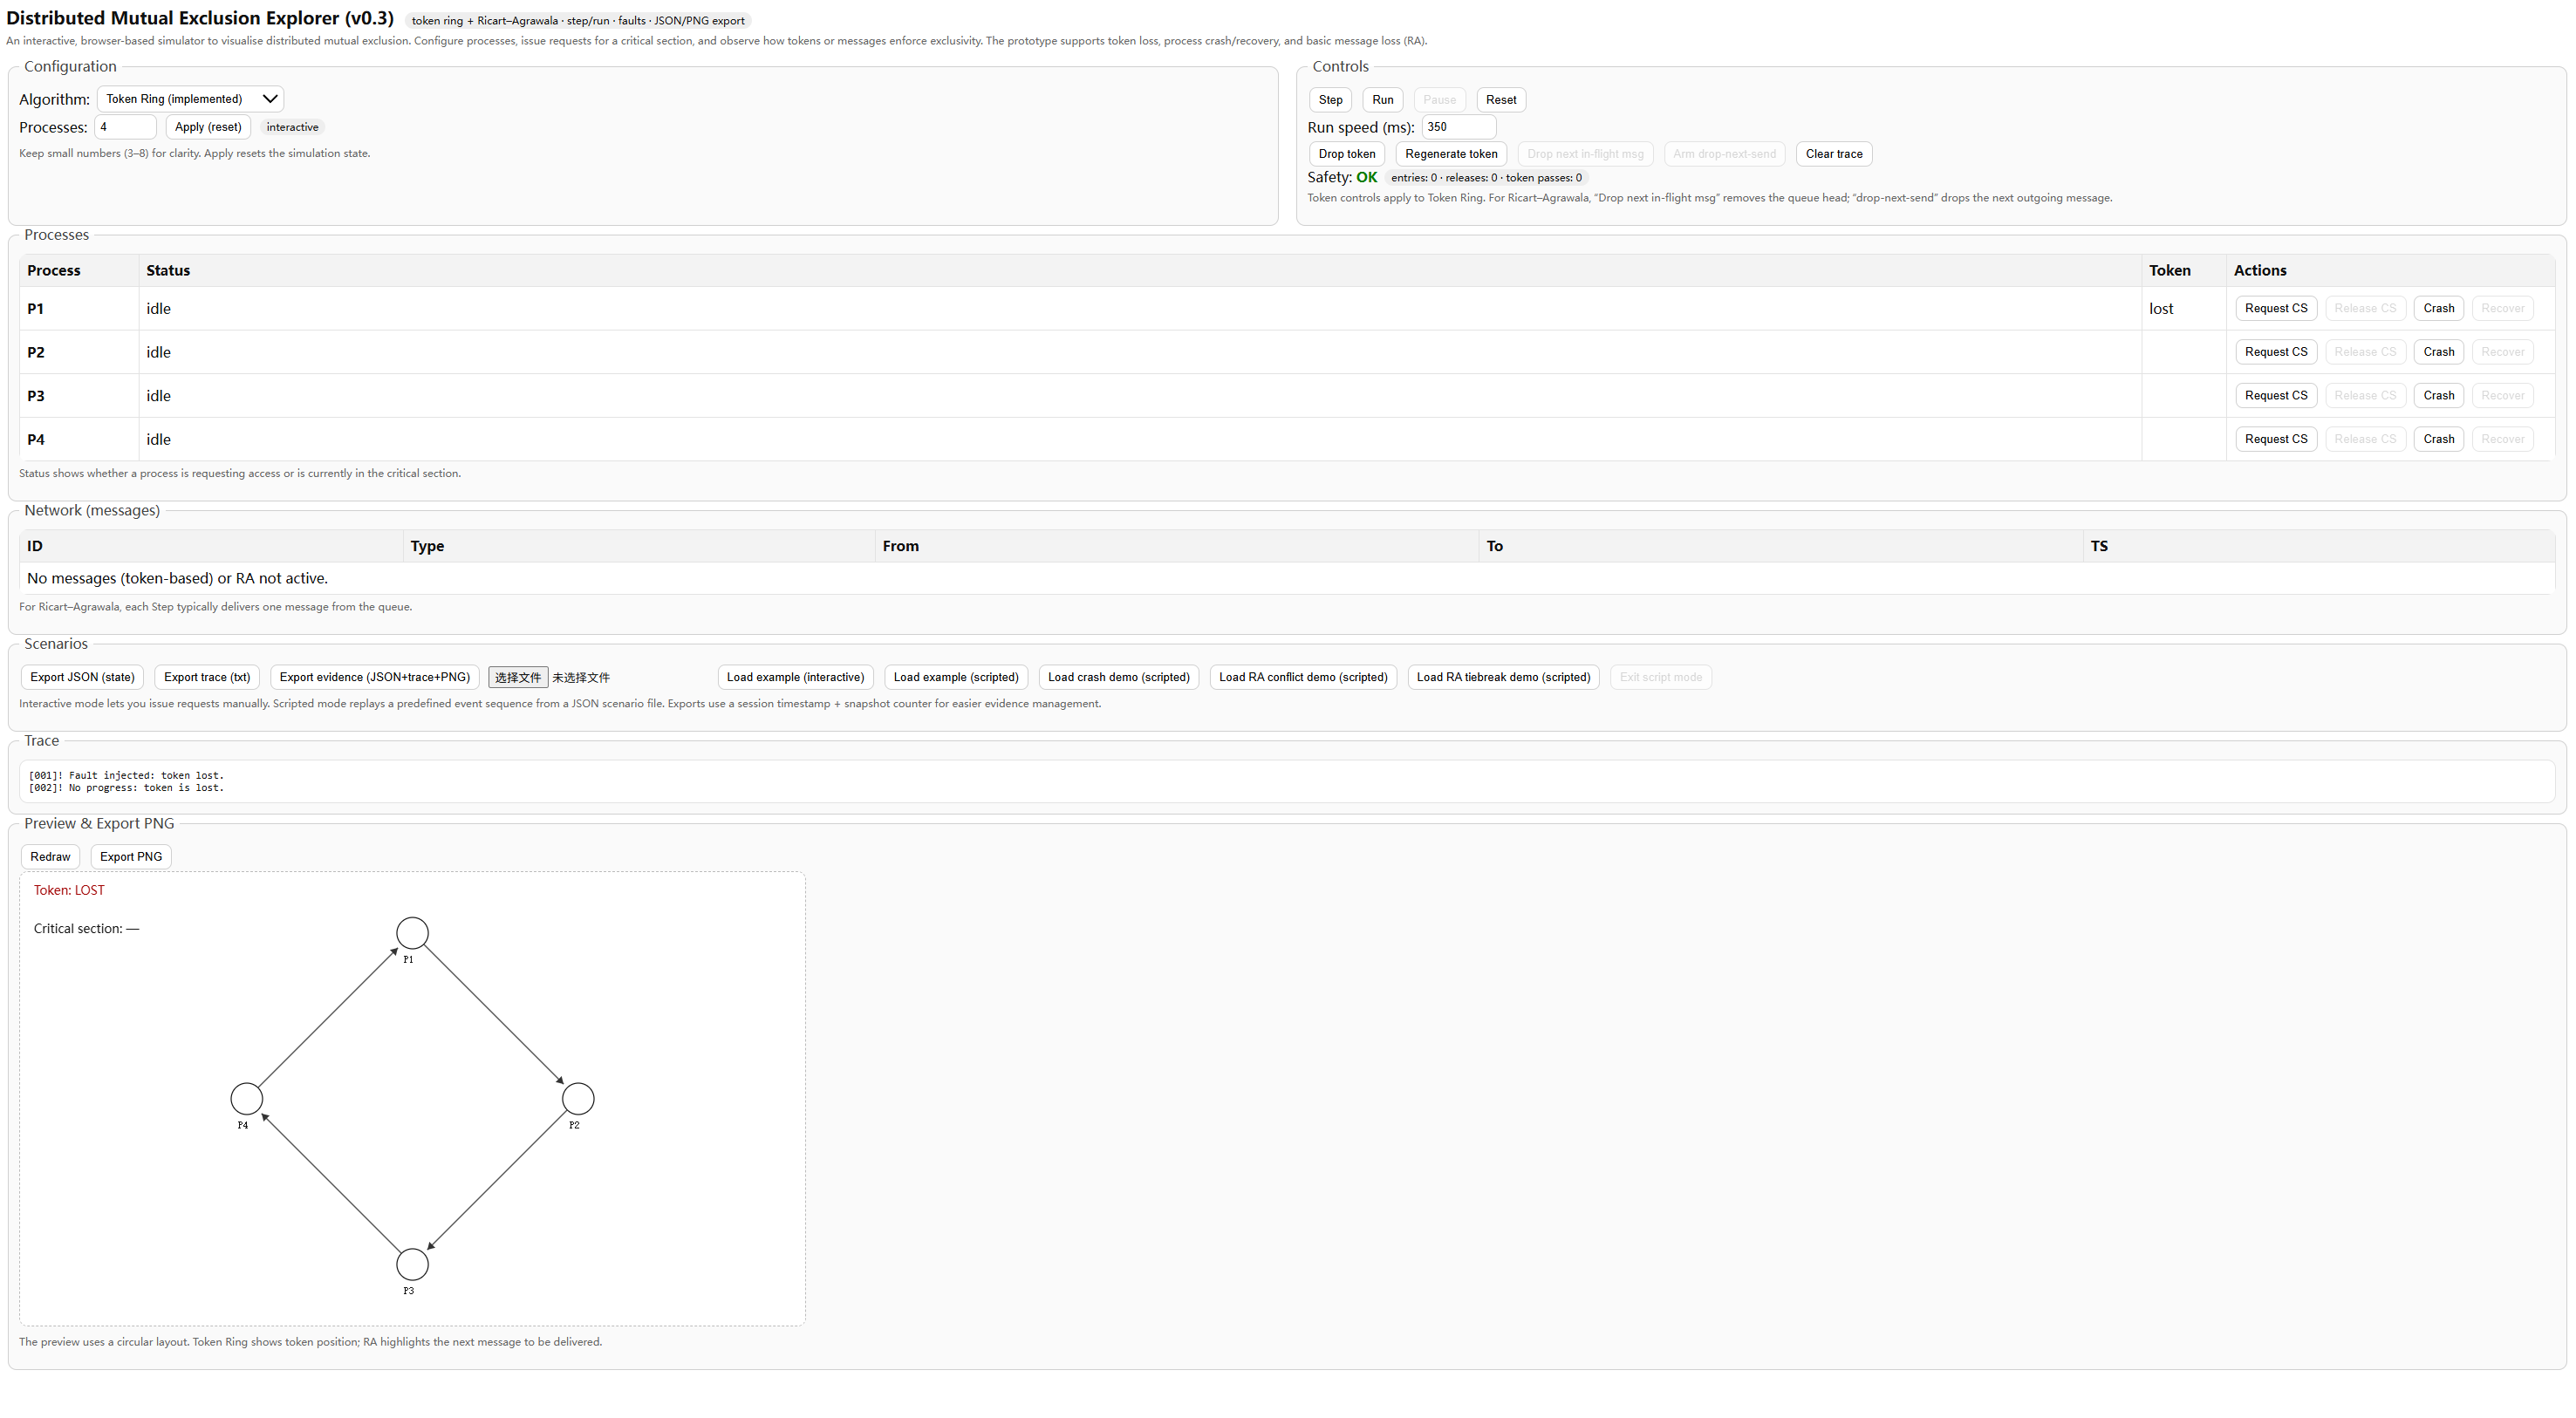
\includegraphics[width=0.82\linewidth]{fig_tr_token_lost.png}
\caption{Token Ring: token loss halts progress until regeneration is performed.}
\label{fig:tr-token-lost}
\end{figure}

\begin{figure}[htbp]
\centering
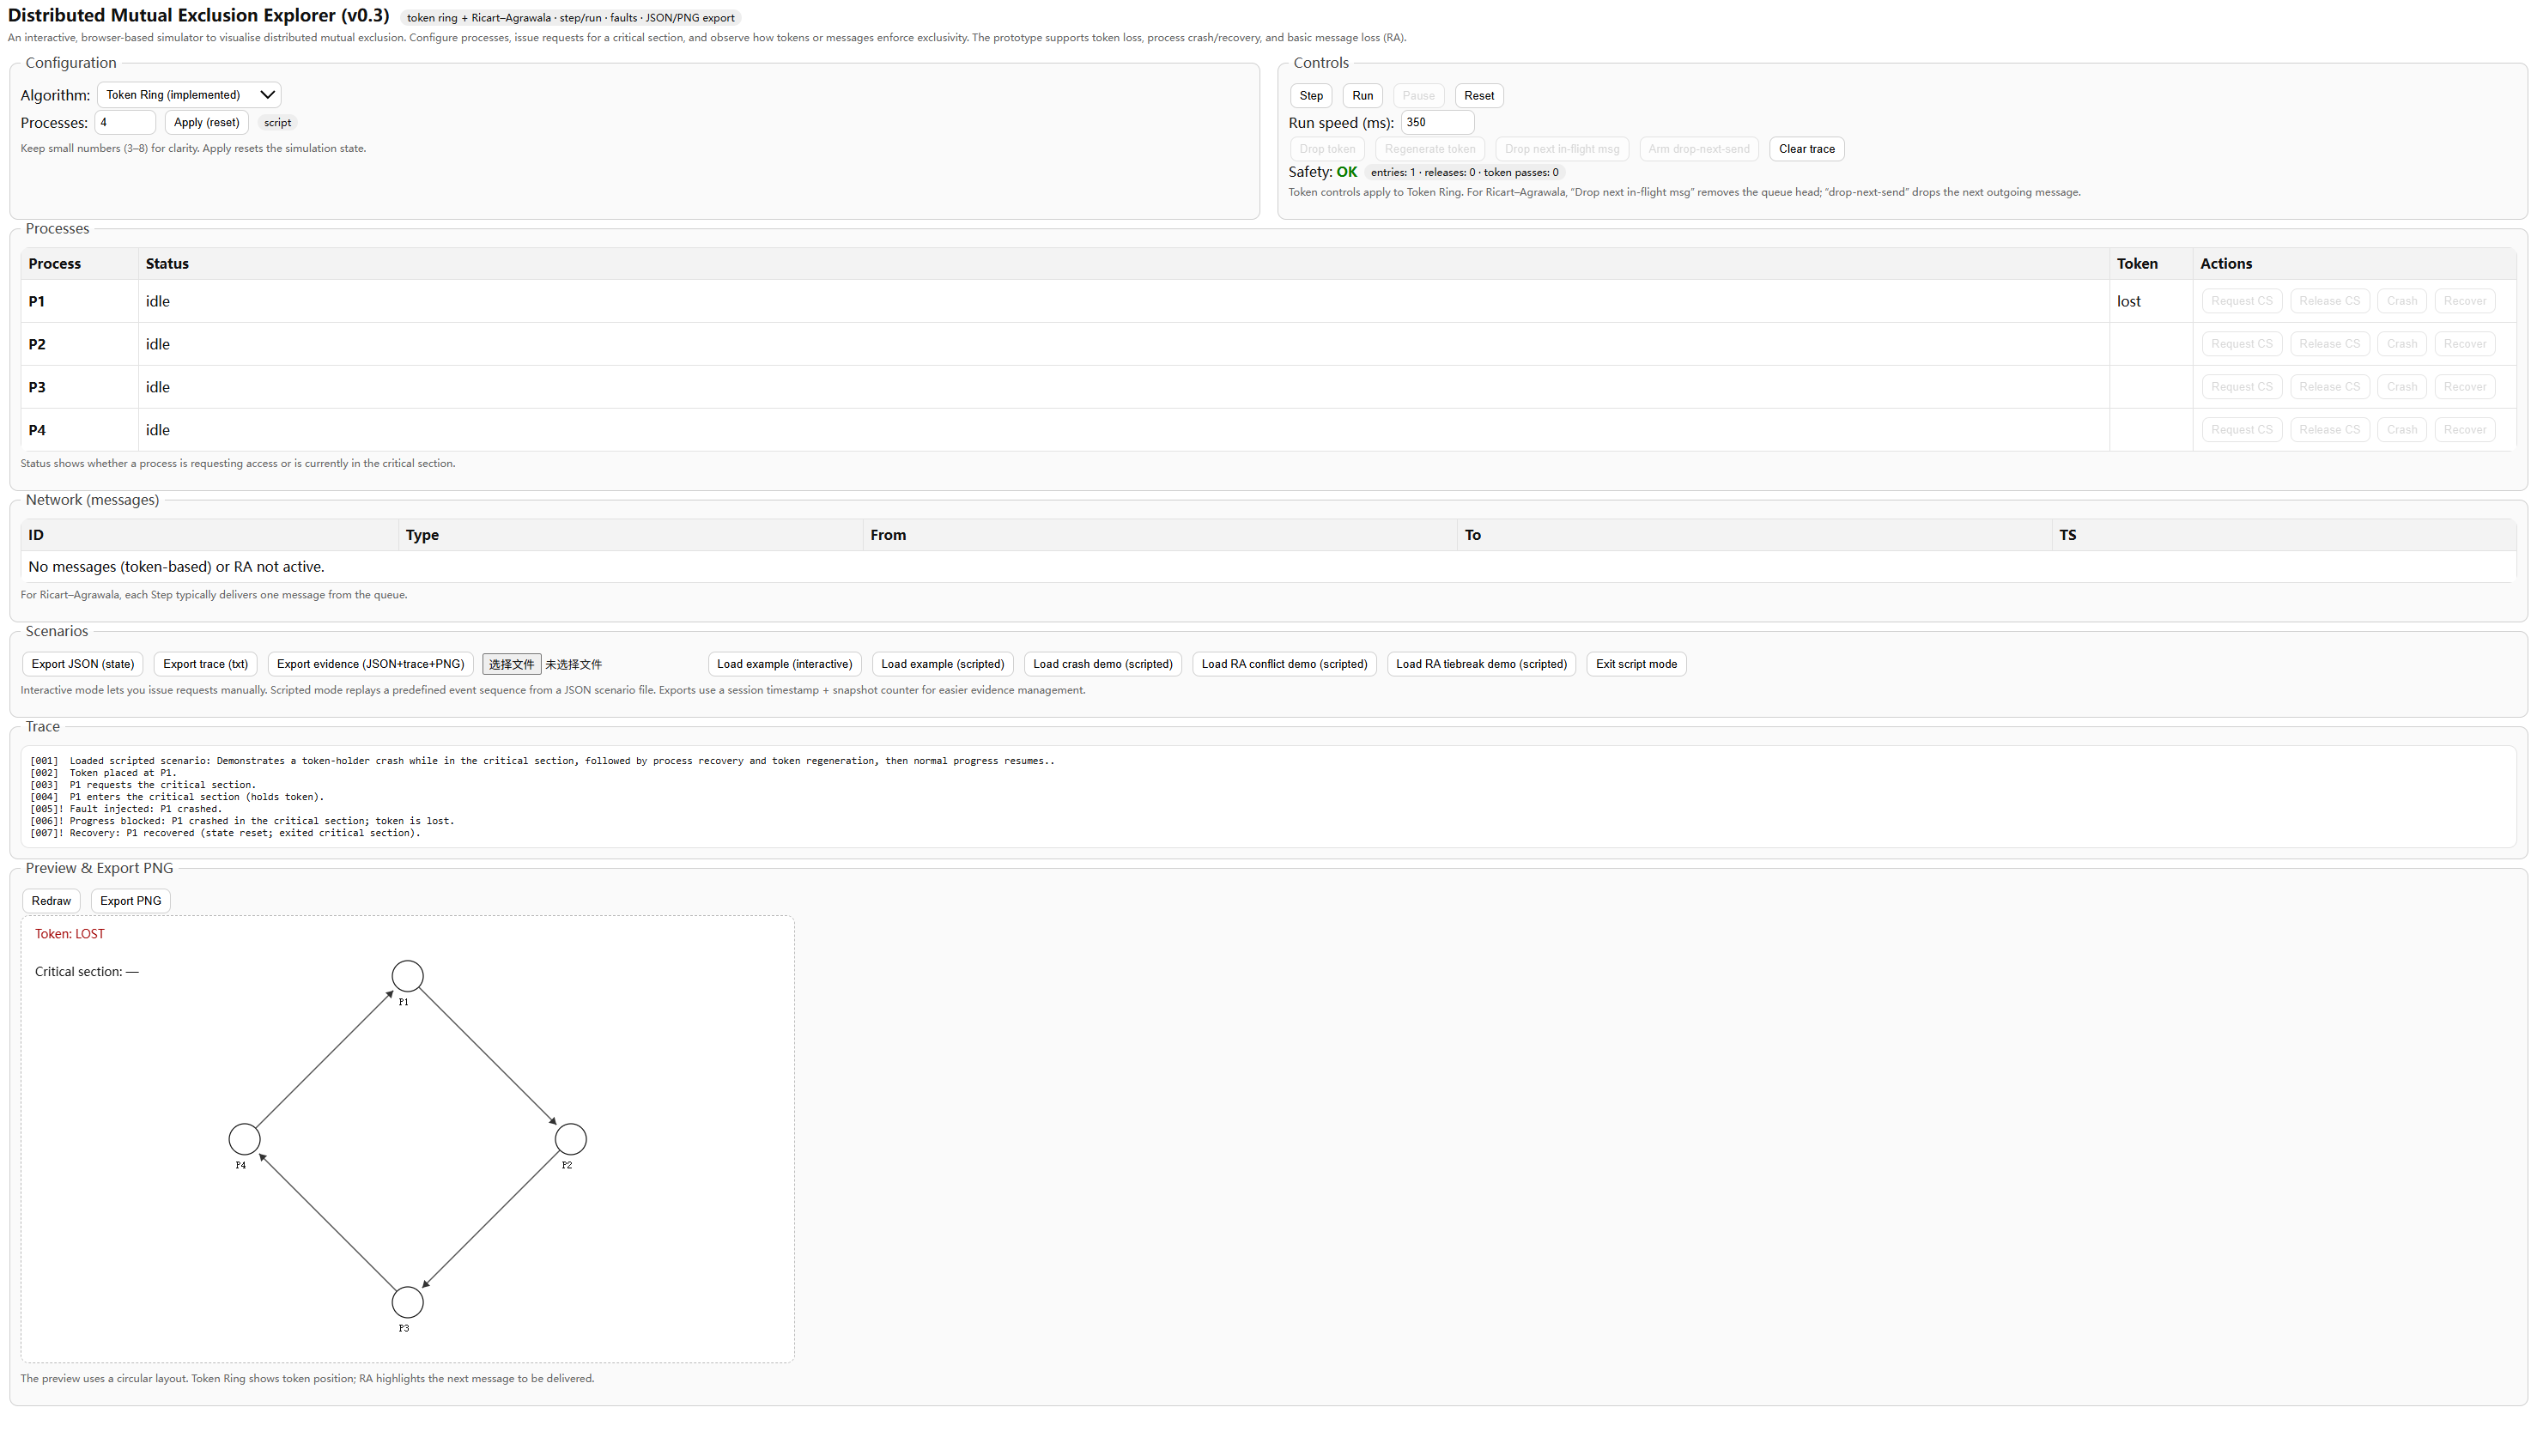
\includegraphics[width=0.82\linewidth]{fig_tr_crash_recover.png}
\caption{Token Ring: crash and recover demonstration.}
\label{fig:tr-crash-recover}
\end{figure}

\subsection{RA Tie-break Behaviour}
A scripted tie-break scenario demonstrates deterministic ordering when requests share the same logical timestamp. Numeric PID ordering is used to resolve the tie, ensuring a stable and explainable outcome \cite{lamport1978time,ricart1981optimal}.

\begin{figure}[htbp]
\centering
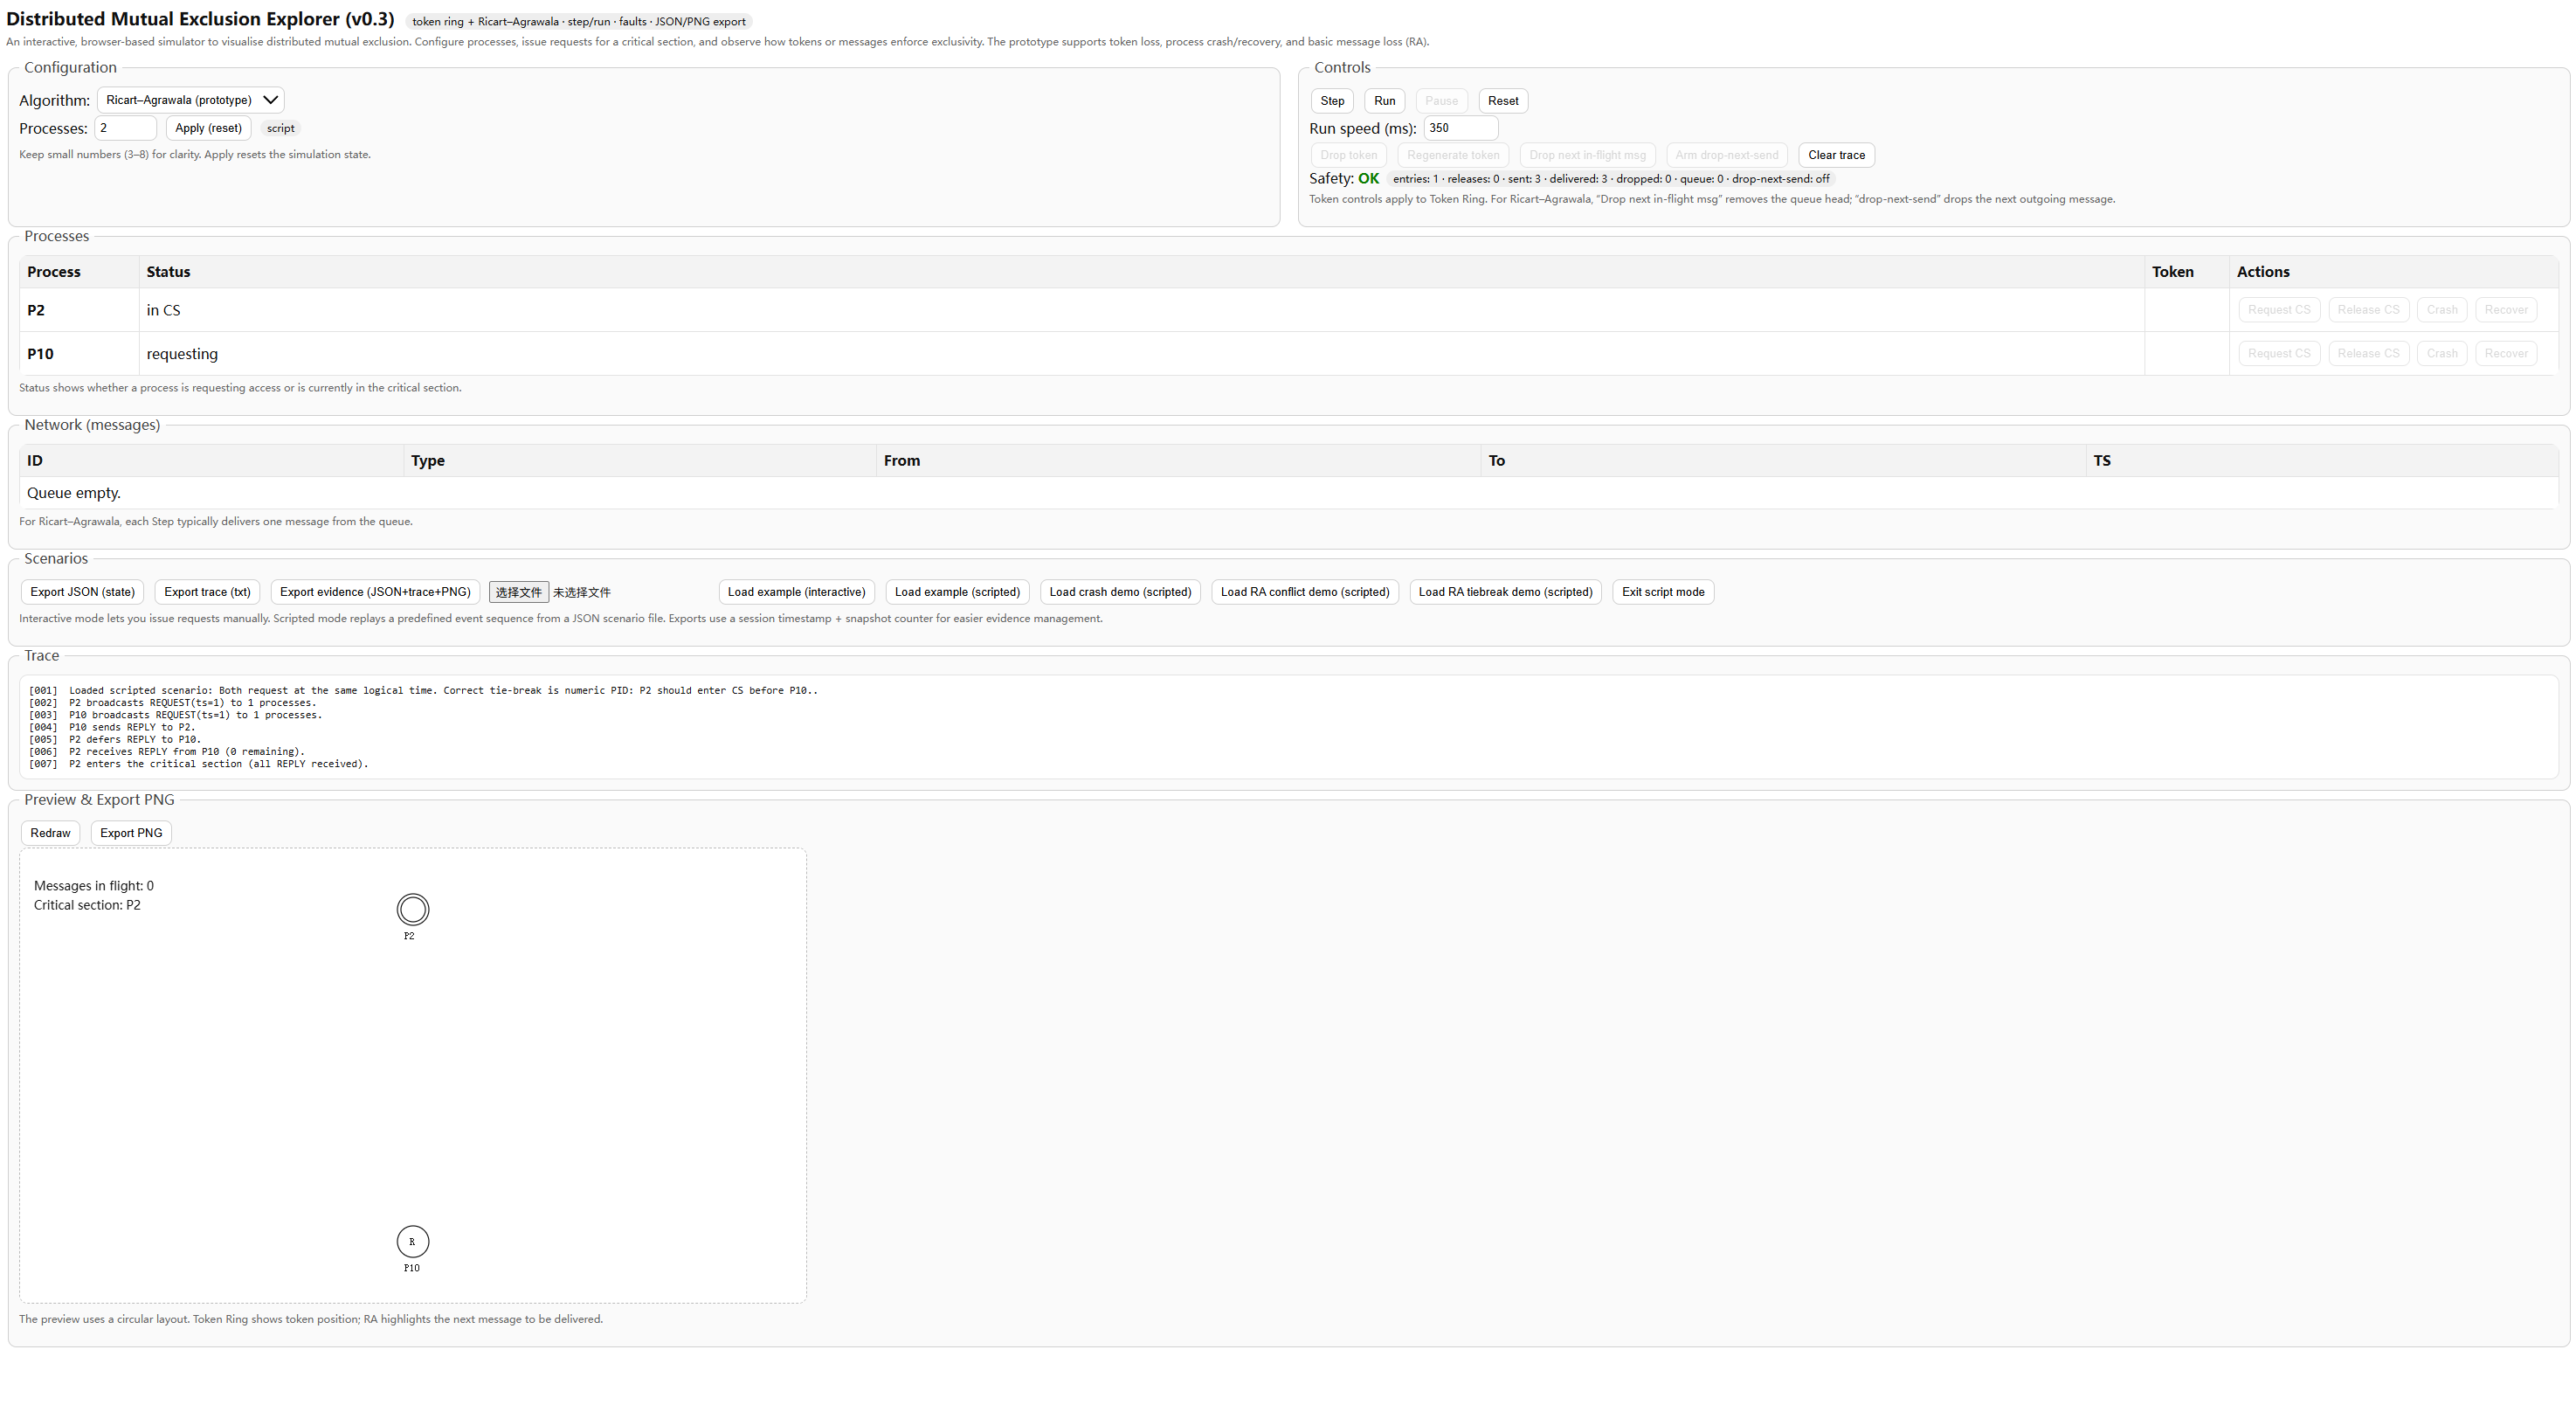
\includegraphics[width=0.82\linewidth]{fig_ra_tiebreak.png}
\caption{RA scripted tie-break case: equal timestamps are resolved deterministically using numeric PID ordering.}
\label{fig:ra-tiebreak}
\end{figure}

\section{Fault Demonstrations: Safety vs Liveness}
The most pedagogically significant result is the explicit separation between safety and liveness. In the RA prototype, message loss can prevent a process from collecting all required REPLY messages, so progress may halt while mutual exclusion remains preserved \cite{lynch1996distributed}.

\subsection{RA-03: Drop Next In-Flight Message}
RA-03 demonstrates network-side message loss. Figure~\ref{fig:ra-drop-inflight} shows the stalled global state after dropping an in-flight message. The figure shows the overall state of the system, while the trace excerpt below identifies the specific missing dependency.

\begin{figure}[htbp]
\centering
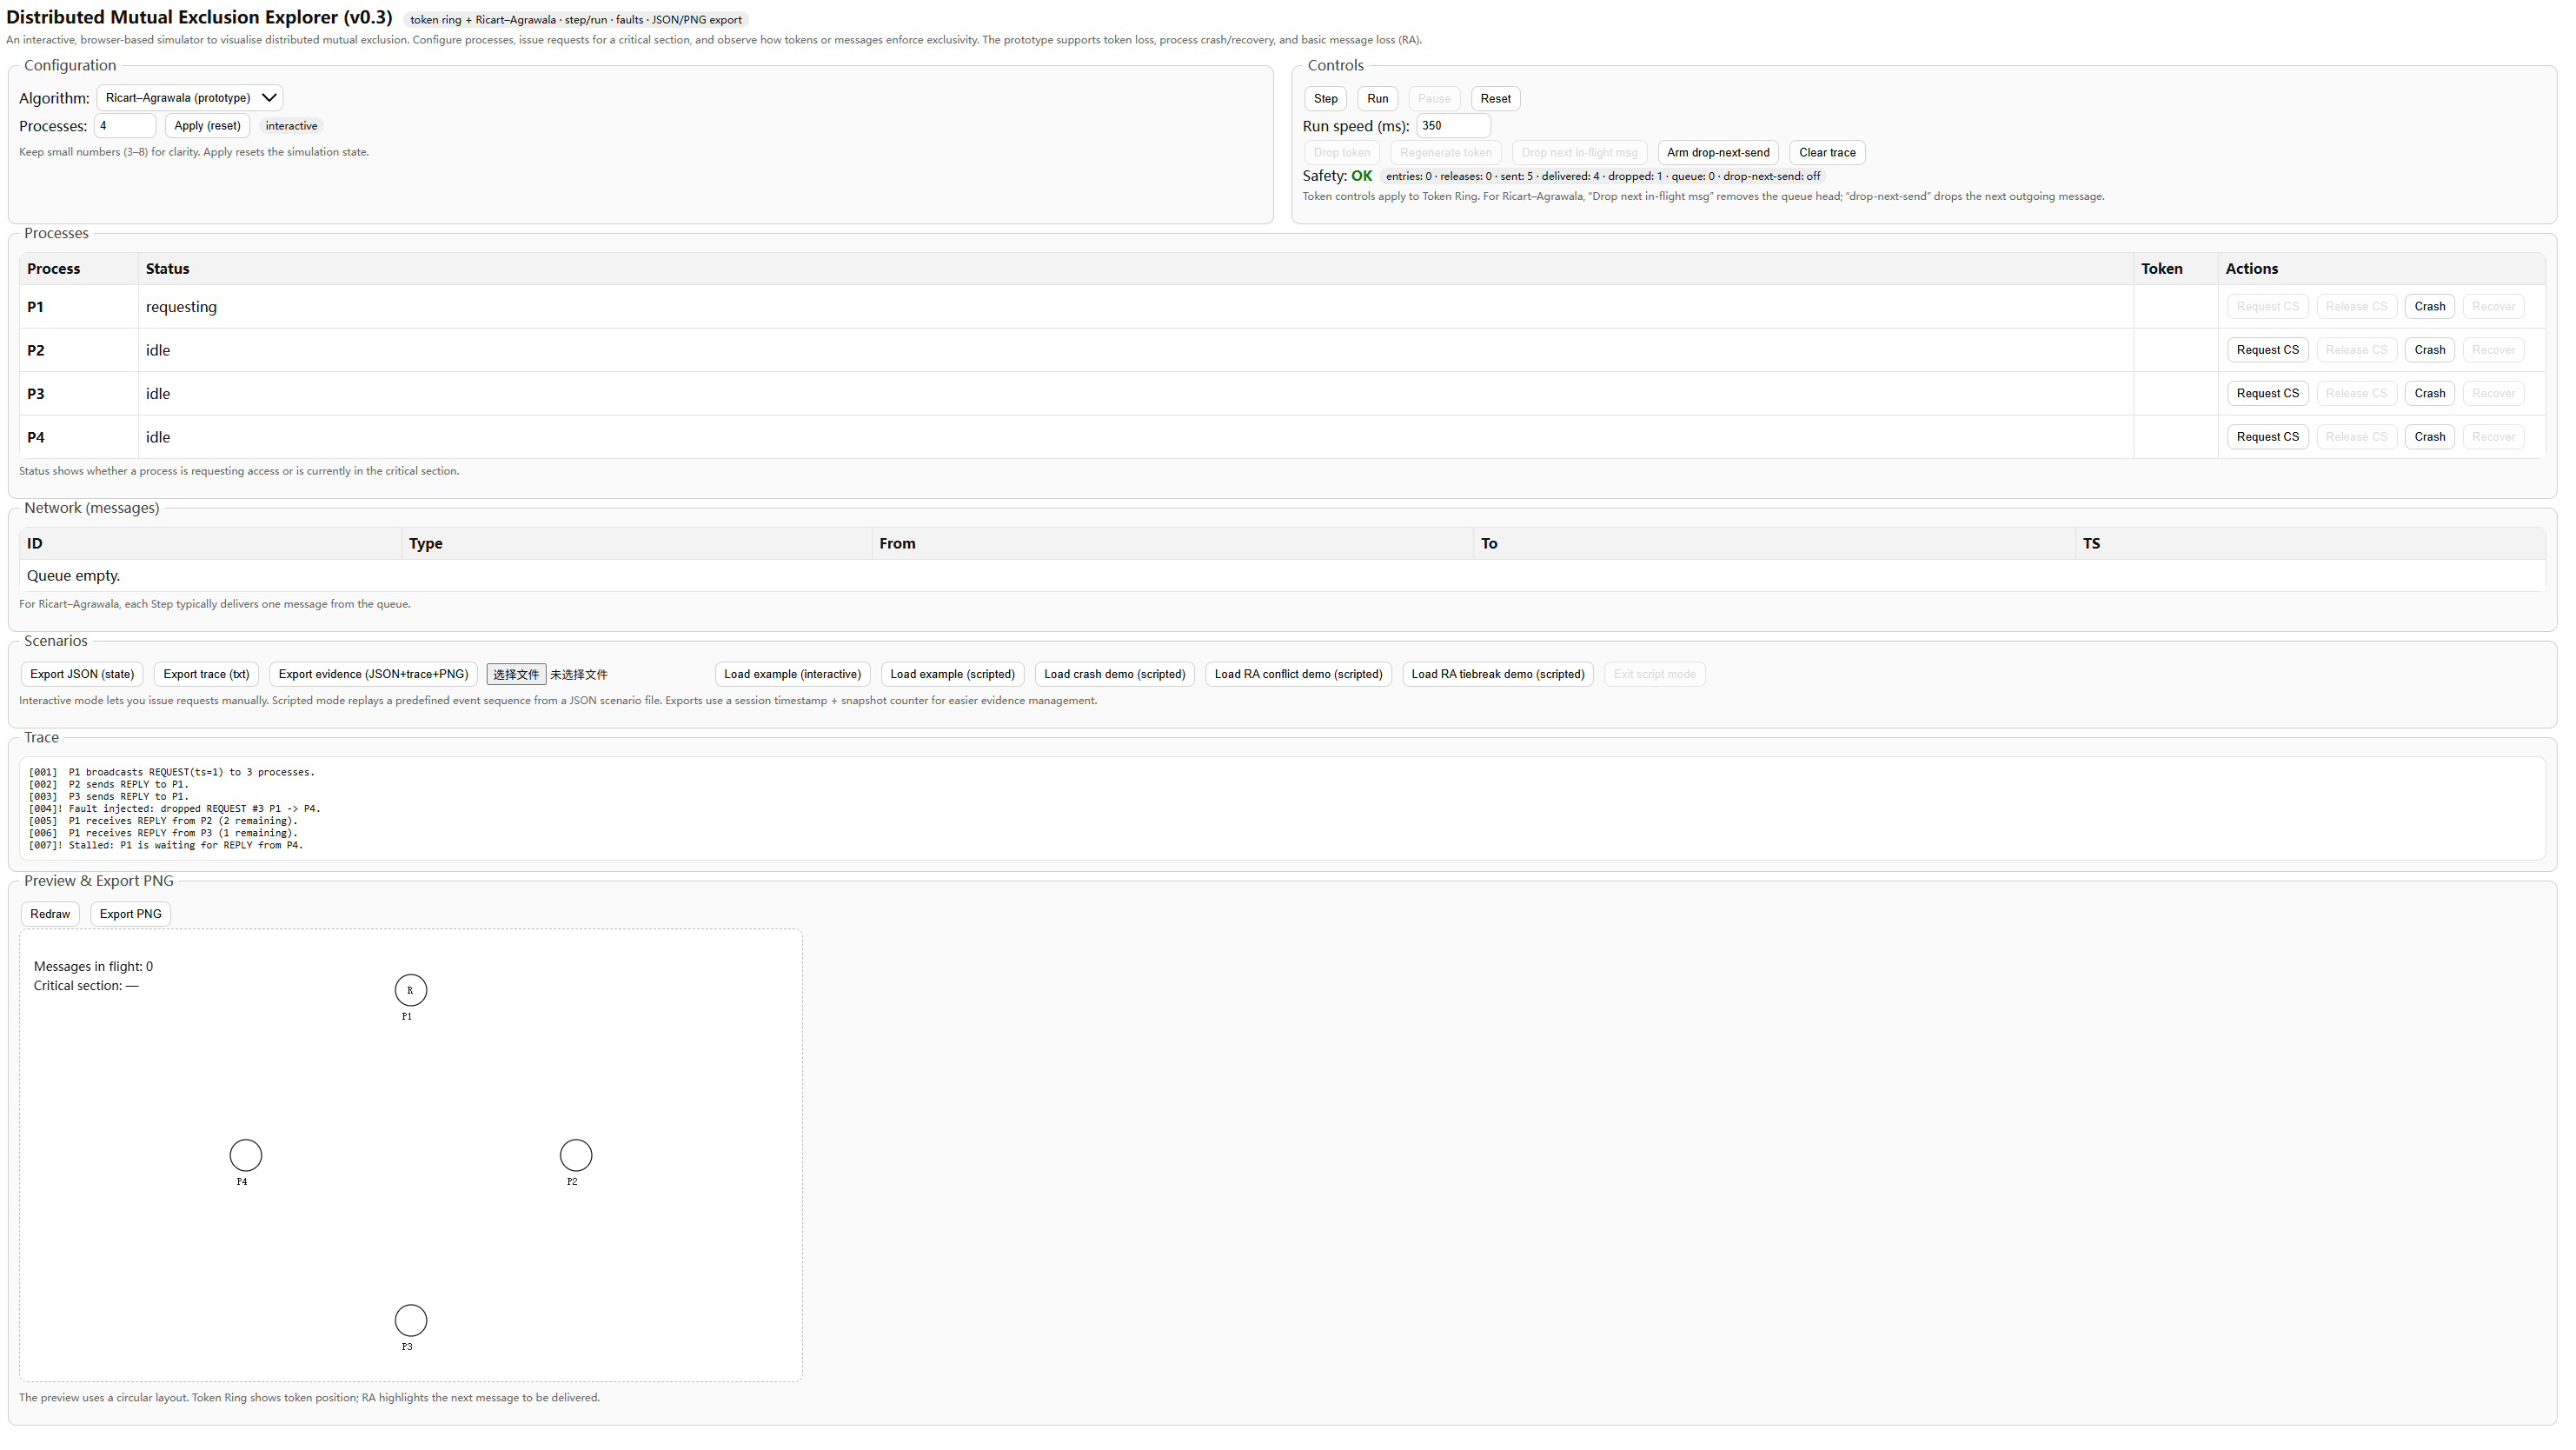
\includegraphics[width=0.82\linewidth]{fig_ra_drop_inflight_stall.png}
\caption{RA stalled state after dropping an in-flight message; see the trace excerpt below for the missing REPLY dependency.}
\label{fig:ra-drop-inflight}
\end{figure}

\begin{verbatim}
Fault injected: dropped REQUEST #3 P1 -> P4.
Stalled: P1 is waiting for REPLY from P4.
\end{verbatim}

This case demonstrates that progress can fail without violating mutual exclusion. The artefact therefore helps learners separate the notion of a correct safety property from the distinct question of eventual progress.

\subsection{RA-04: Drop-Next-Send}
RA-04 demonstrates send-side message loss. The resulting global stalled state is shown in Figure~\ref{fig:ra-drop-next-send}, and the trace excerpt below provides the causal explanation.

\begin{figure}[htbp]
\centering
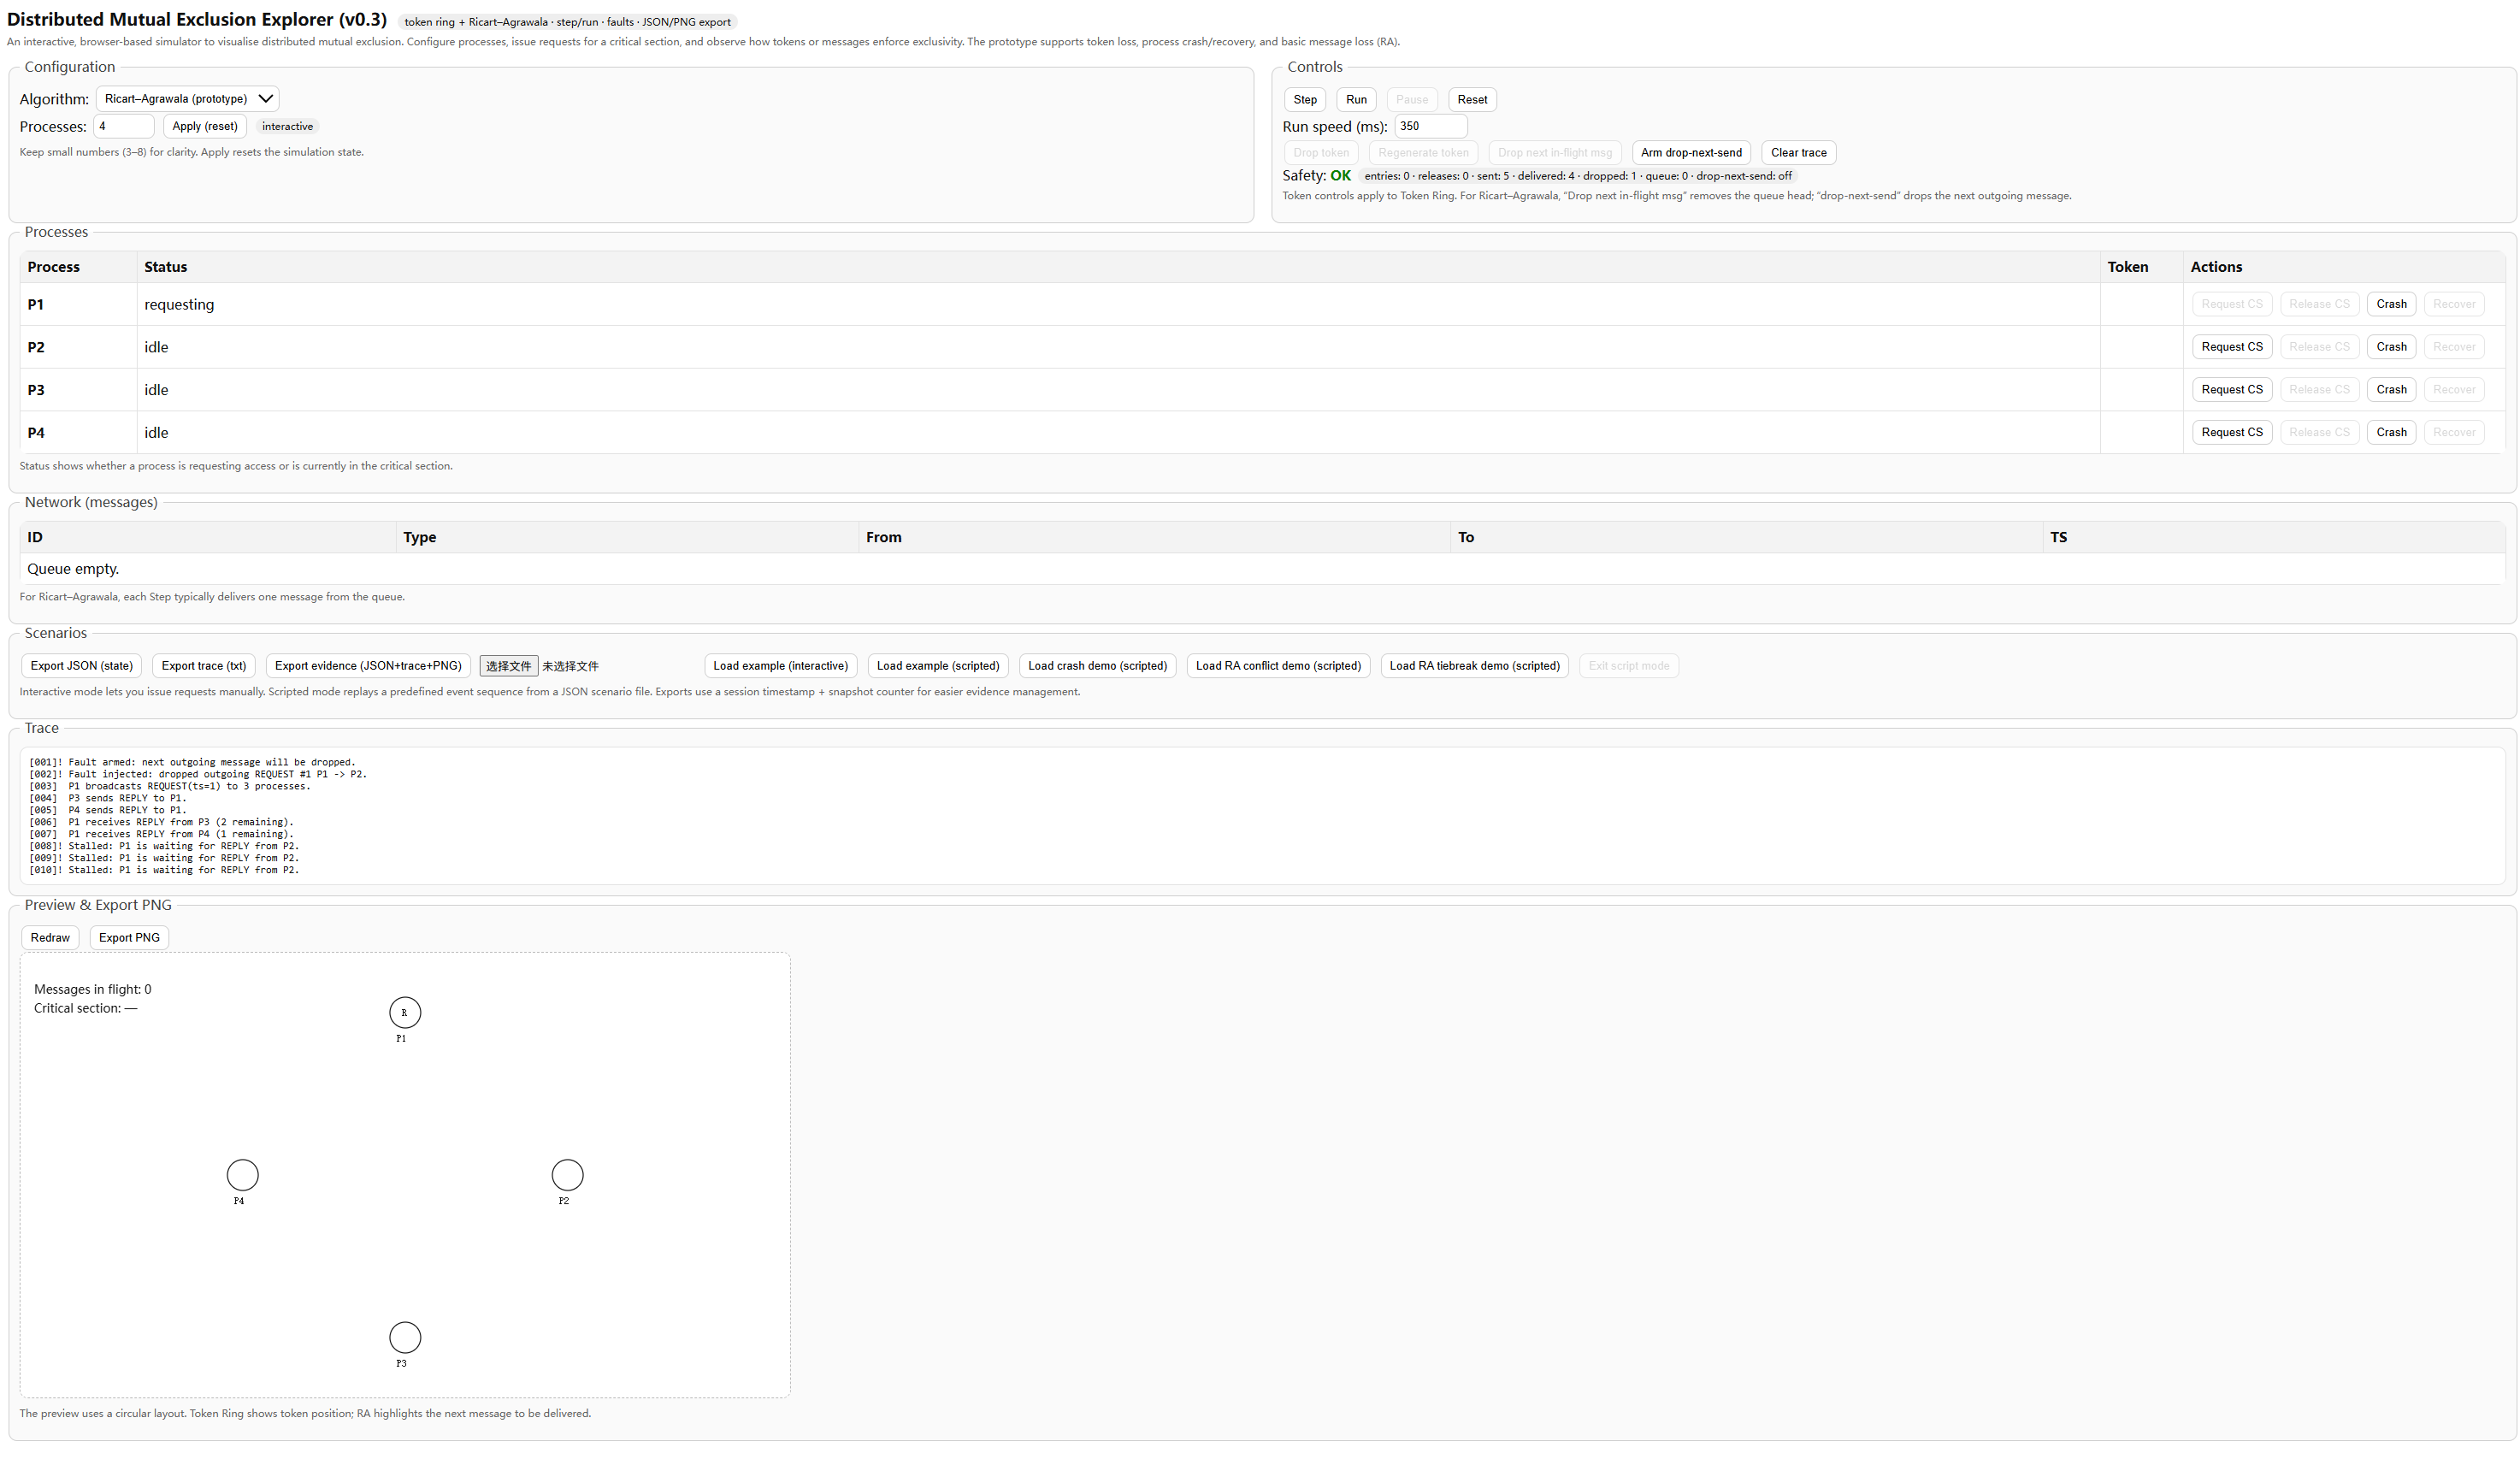
\includegraphics[width=0.82\linewidth]{fig_ra_drop_next_send_stall.png}
\caption{RA stalled state after dropping the next outgoing message; see the trace excerpt below for the missing REPLY dependency.}
\label{fig:ra-drop-next-send}
\end{figure}

\begin{verbatim}
Fault armed: next outgoing message will be dropped.
Fault injected: dropped outgoing REQUEST #1 P1 -> P2.
Stalled: P1 is waiting for REPLY from P2.
\end{verbatim}

Together, RA-03 and RA-04 demonstrate that the artefact is not only useful for showing correct runs, but also for making fault consequences and dependency failures visible.

\section{Usability Evaluation}
Usability was assessed using Nielsen’s heuristic framework \cite{nielsen1994usability}. The updated checklist covers:
\begin{itemize}
  \item algorithm selection,
  \item fault controls,
  \item queue visibility,
  \item trace readability,
  \item and evidence export.
\end{itemize}

Table~\ref{tab:nielsen-summary} summarises the most relevant findings and severity ratings.

\begin{table}[htbp]
\centering
\small
\renewcommand{\arraystretch}{1.15}
\begin{tabular}{p{0.30\linewidth} p{0.12\linewidth} p{0.45\linewidth}}
\toprule
\textbf{Finding} & \textbf{Severity} & \textbf{Interpretation / Action} \\
\midrule
Trace clearly explains state changes and stalls & 1 & Strong learning support; retain as a core feature. \\
Preview symbols may require a legend for new users & 2 & Add a small legend in a future iteration. \\
Fault controls are useful but visually dense & 1 & Current grouping is acceptable; optional advanced toggle later. \\
Algorithm differences are not explained in-app & 2 & Add concise algorithm help text later. \\
Evidence export is useful but not fully self-explanatory to first-time users & 1 & Covered by README and appendices; in-app guidance could be improved. \\
\bottomrule
\end{tabular}
\caption{Summary of key Nielsen heuristic findings (severity scale 0--4).}
\label{tab:nielsen-summary}
\end{table}

Overall, the artefact performs well on visibility of system status, user control, and fault explainability. Remaining usability work is concentrated in discoverability and lightweight in-app guidance rather than in the correctness of interaction.

\section{Reproducibility}
Reproducibility is a major strength of the project. It is supported by:
\begin{itemize}
  \item a freeze baseline tag and release,
  \item CI-backed automated tests,
  \item evidence triplet exports,
  \item evidence and figure indices,
  \item and a consistent local run method.
\end{itemize}

A compact reproducibility protocol is:
\begin{enumerate}
  \item checkout tag \texttt{v0.3.2},
  \item run \texttt{python -m http.server 5500},
  \item open the local URL,
  \item load the relevant demo or perform the manual case steps,
  \item export the evidence triplet,
  \item compare the exported trace and preview against the report references.
\end{enumerate}

This turns reproducibility into an executable process rather than a rhetorical claim \cite{sandve2013ten,wilson2014best,wilkinson2016fair}.

\section{Threats to Validity}
The evaluation has several limitations:
\begin{itemize}
  \item the queue-based network is a teaching abstraction rather than a high-fidelity asynchronous model,
  \item RA is intentionally presented as a teaching-oriented prototype rather than a full fault-tolerant protocol,
  \item usability was evaluated heuristically rather than through a substantial participant study.
\end{itemize}

These limitations are documented explicitly to avoid overstating the scope of the conclusions.

\section{Summary}
The evaluation shows that the artefact meets its educational objectives:
\begin{itemize}
  \item safety is preserved across tested scenarios,
  \item fault injection successfully illustrates progress and liveness trade-offs,
  \item usability is strong in visibility and control,
  \item and reproducible evidence can be generated and audited.
\end{itemize}

The combined result is not merely a working simulator, but a reportable and inspectable educational artefact.}{}
\IfFileExists{Chapters/07_professional_issues.tex}{\chapter{Professional Issues}
\label{ch:professional}

\section{Overview}
Final-year computing projects are expected to address not only technical correctness, but also the broader professional issues that shape responsible software development. For this project, the most relevant issues are:
\begin{itemize}
  \item accessibility,
  \item privacy and data handling,
  \item sustainability and maintainability,
  \item reproducibility and research integrity,
  \item and ethics in evaluation and communication.
\end{itemize}

These issues are particularly important because the artefact is intended as an educational tool: its value depends not only on whether it works, but also on whether it can be used, trusted, maintained, and interpreted responsibly.

\section{Accessibility}
Accessibility is an important professional responsibility for educational software. A tool designed to support learning should not unnecessarily exclude users because of avoidable interface barriers. Current accessibility-relevant strengths of the artefact include:
\begin{itemize}
  \item explicit textual status indicators (for example, process states, the Safety indicator, and trace messages),
  \item grouped controls with consistent action labels,
  \item and the use of multiple views (tables, trace, preview) so that critical information is not conveyed only through a single visual channel.
\end{itemize}

These design choices are helpful, but they do not by themselves guarantee accessibility. Relative to accessibility guidance such as WCAG 2.2 and ARIA recommendations \cite{w3c_wcag22,w3c_aria12}, several limitations remain:
\begin{itemize}
  \item the interface has not been systematically evaluated for keyboard-only navigation,
  \item screen-reader behaviour has not been formally tested,
  \item and some visual markers in the preview (for example, the request marker, token indicator, and crash marker) may still benefit from a compact legend or additional textual equivalents.
\end{itemize}

Accordingly, the current position of the project is that accessibility has been considered at a basic practical level, but there remains clear scope for improvement in a future iteration. This is acceptable for a prototype, provided the limitation is stated explicitly.

\section{Privacy and Data Handling}
The privacy implications of the artefact are limited, because the simulator is designed to run locally or as a static web page and does not require user accounts or server-side storage. By default:
\begin{itemize}
  \item no personal data are collected,
  \item no analytics are embedded,
  \item and exported JSON/trace/PNG files contain only simulation state and evidence data.
\end{itemize}

This is a positive design choice because it reduces risk and simplifies both deployment and explanation. However, privacy still matters at the level of workflow and reporting. If screenshots, traces, or future participant feedback are collected, these materials should be managed carefully and stored only where necessary. In the current project, all evidence is technical rather than personal, which keeps privacy concerns low.

\section{Ethics and Research Governance}
No formal human-subject study was conducted as part of the current evaluation. The evaluation therefore remains within a low-risk scope based on:
\begin{itemize}
  \item manual evidence-driven testing,
  \item heuristic usability inspection,
  \item and automated testing of the artefact itself.
\end{itemize}

This is an important point for research governance: the current report does not make claims based on participant data, and therefore does not present the artefact as having been validated through a controlled human study.

If the project were extended to include participant-based evaluation (for example, a structured comparison of learner performance or a SUS questionnaire), appropriate ethical safeguards would be required. These would include:
\begin{itemize}
  \item informed consent,
  \item data minimisation,
  \item anonymisation where appropriate,
  \item and compliance with the university’s relevant ethics procedures.
\end{itemize}

Stating this boundary clearly avoids over-claiming the scope of the present evaluation.

\section{Sustainability and Maintainability}
A major professional consideration for software artefacts is whether they remain maintainable over time. In this project, sustainability was addressed through several practical engineering choices:
\begin{itemize}
  \item the artefact is dependency-free and browser-based,
  \item the codebase is intentionally small,
  \item the core simulation engine is separated from the UI layer,
  \item and version control plus tagged releases provide traceability.
\end{itemize}

These choices reduce the likelihood of build breakage due to external dependency drift and make the system easier to understand and evolve. In this sense, the project adopts a deliberately conservative architecture in order to improve long-term robustness \cite{chacon2014progit,wilson2014best}.

At the same time, maintainability is not only a question of code structure. It also depends on whether decisions are documented and whether testing protects against regressions. The inclusion of smoke tests, unit tests, evidence indices, and release notes therefore contributes directly to maintainability.

\section{Reproducibility and Research Integrity}
Reproducibility is one of the strongest professional aspects of the project. Rather than treating reproducibility as an optional afterthought, the project integrates it into the artefact workflow itself. Specifically:
\begin{itemize}
  \item the project defines a freeze baseline release,
  \item evidence is exported as a triplet (state JSON, trace TXT, preview PNG),
  \item evidence indices and figure indices map report claims to raw artefacts,
  \item and CI-backed smoke tests provide automated regression checks.
\end{itemize}

This supports research integrity in two ways. First, it makes the evaluation claims auditable. Second, it reduces the risk that report figures and conclusions become detached from the actual implementation \cite{sandve2013ten,wilson2014best,wilkinson2016fair}.

A related issue is honest communication of uncertainty. The report explicitly distinguishes between:
\begin{itemize}
  \item what is demonstrated empirically,
  \item what is inferred from those demonstrations,
  \item and what remains out of scope.
\end{itemize}
For example, the Ricart--Agrawala implementation is described as a teaching-oriented prototype rather than a fully fault-tolerant production protocol. This is not merely a wording choice; it is part of maintaining professional and academic integrity.

\section{Responsible Communication of Limitations}
A professional report should make limitations clear rather than hide them. This project has several important limitations:
\begin{itemize}
  \item the network is modelled as a queue-based teaching abstraction,
  \item retransmission and failure detectors are not implemented,
  \item usability evaluation is heuristic rather than participant-based,
  \item and some accessibility aspects remain future work.
\end{itemize}

These limitations are not failures of the project; rather, they are part of its scope definition. The responsible approach is to explain them clearly and to avoid making claims that would imply a stronger validation or a more realistic distributed environment than the project actually provides.

\section{Professional Standards and Evaluation Practice}
Usability discussion in this report is informed by Nielsen’s heuristics \cite{nielsen1994usability} and broader usability concepts from ISO 9241-11 \cite{iso9241_11_2018}. These frameworks help anchor the evaluation in recognised professional practice. Similarly, reproducibility and version-control choices align the project with established norms in research software development \cite{sandve2013ten,wilson2014best,chacon2014progit}.

\section{Summary}
The professional issues analysis shows that the project is not only technically competent, but also developed with attention to responsible software practice. Its main strengths are low privacy risk, strong reproducibility, and a maintainable architecture. Its main limitations lie in accessibility completeness and the absence of participant-based evaluation. These are acceptable for the current scope, provided they are documented transparently and treated as priorities for future work.}{}
\IfFileExists{Chapters/08_conclusion.tex}{\chapter{Conclusion and Future Work}
\label{ch:conclusion}

\section{Conclusion}
This project set out to develop an interactive educational artefact for learning distributed mutual exclusion. The resulting system, the \emph{Distributed Mutual Exclusion Explorer}, provides a browser-based environment in which learners can observe and manipulate two representative coordination approaches:
\begin{itemize}
  \item a token-based Token Ring model,
  \item and a message-based Ricart--Agrawala (RA) teaching-oriented prototype.
\end{itemize}

The central achievement of the project is not the invention of a new algorithm, but the creation of a tool that makes the behaviour of distributed mutual exclusion visible, explainable, and reproducible. In particular, the artefact supports:
\begin{itemize}
  \item step-by-step execution,
  \item scripted demos,
  \item fault injection and recovery,
  \item trace-based explanations,
  \item and exportable evidence suitable for report-based evaluation.
\end{itemize}

From a correctness perspective, the project demonstrates the preservation of the mutual exclusion safety invariant across the tested scenarios. From an educational perspective, the artefact is especially strong in making the distinction between \emph{safety} and \emph{liveness} concrete. This is most visible in the RA message-loss cases, where the tool does not simply fail silently, but instead explains why progress has stalled.

The project also makes a contribution at the level of engineering and reproducibility. By combining:
\begin{itemize}
  \item a freeze baseline release,
  \item automated smoke and unit testing,
  \item evidence triplet export,
  \item and indexed mappings between figures and evidence,
\end{itemize}
the project supports a report workflow in which claims are traceable back to concrete artefacts. This strengthens the credibility of the written evaluation and aligns the project with professional software and research practices.

\section{Achievement Against Objectives}
The objectives stated in Chapter~\ref{ch:introduction} have been substantially met.

\begin{itemize}
  \item A technically correct simulation preserving the mutual exclusion safety property was implemented.
  \item Step-by-step execution and explanatory traces were provided for both algorithms.
  \item Token-based and message-based mutual exclusion were both represented.
  \item Fault injection and recovery mechanisms were added and evaluated.
  \item Reproducible evidence export and indexing were integrated into the workflow.
  \item Correctness, usability, and reproducibility were evaluated through structured methods.
\end{itemize}

Taken together, these outcomes mean that the project satisfies the main educational and technical aims of Variant 3.

\section{Main Limitations}
Several limitations remain and should be recognised explicitly.

First, the RA component is intentionally a \emph{teaching-oriented prototype}. It does not attempt to model all aspects of realistic distributed communication, such as retransmission, timeouts, or failure detectors. Second, the network representation is deliberately simplified into a queue-based model to support visibility and reproducibility. Third, usability was assessed heuristically rather than through a large participant study. Finally, while accessibility has been considered, it has not yet been evaluated systematically.

These limitations do not invalidate the project, but they define its scope and should guide how its contributions are interpreted.

\section{Future Work}
Several directions for future work follow naturally from the current artefact.

\subsection{Algorithmic Extensions}
The current system focuses on Token Ring and RA because they provide a strong contrast between token-based and message-based coordination. Future work could add:
\begin{itemize}
  \item Suzuki--Kasami for a richer token-based comparison \cite{suzuki1985distributed},
  \item Maekawa to illustrate quorum-based trade-offs \cite{maekawa1985sqrt},
  \item or Raymond’s algorithm for a more structured token-routing approach \cite{raymond1989tree}.
\end{itemize}

\subsection{Fault-Tolerance Extensions}
For RA in particular, a natural next step would be to add optional recovery-oriented mechanisms such as:
\begin{itemize}
  \item timeouts,
  \item retransmissions,
  \item or simplified failure-detector logic \cite{chandra1996failure}.
\end{itemize}

This would allow the tool to contrast \emph{pure algorithmic assumptions} with \emph{fault-tolerant engineering extensions}.

\subsection{Interface and Accessibility Improvements}
Several usability and accessibility improvements are also realistic:
\begin{itemize}
  \item a legend for preview symbols,
  \item concise in-app algorithm explanations,
  \item keyboard shortcuts,
  \item and stronger keyboard/screen-reader support aligned with WCAG and ARIA guidance \cite{w3c_wcag22,w3c_aria12}.
\end{itemize}

\subsection{User Study and Stronger Educational Validation}
A future iteration could extend the current heuristic evaluation with a participant-based study. This might include:
\begin{itemize}
  \item structured learner tasks,
  \item pre-/post-task conceptual questions,
  \item or a lightweight usability instrument such as SUS \cite{brooke1996sus}.
\end{itemize}

This would strengthen claims about pedagogical effectiveness beyond the current evidence-driven and heuristic framework.

\section{Final Reflection}
The final outcome of the project is a working and evaluable teaching artefact that makes an abstract area of distributed systems more concrete. It demonstrates that meaningful final-year project work in computing is not limited to building a technically functioning system; it also involves creating something that can be reasoned about, tested, evaluated, and communicated responsibly. In that sense, the project succeeds both as a software artefact and as a piece of engineering-led academic work.}{}

% ------------------------------------------------------------
% Bibliography
% ------------------------------------------------------------
\bibliographystyle{unsrtnat}
\bibliography{references}

% ------------------------------------------------------------
% Appendices
% ------------------------------------------------------------
\appendix
\IfFileExists{Appendices/A_user_manual.tex}{\chapter{User Manual}
\label{app:user-manual}

\section{Running the Tool Locally}
From the repository root, start a local server:
\begin{verbatim}
python -m http.server 5500
\end{verbatim}
Open:
\begin{verbatim}
http://localhost:5500/
\end{verbatim}

\section{Basic Usage}
\begin{itemize}
  \item Select an algorithm (Token Ring or RA) and choose the number of processes.
  \item Use \textbf{Request CS} to issue a request.
  \item Use \textbf{Step} to progress deterministically.
  \item Use \textbf{Run/Pause} for automated playback.
  \item Observe the process table, message queue table, trace, safety label, and preview canvas.
\end{itemize}

\section{Fault Injection}
\begin{itemize}
  \item Token Ring: use \textbf{Drop token}, \textbf{Regenerate token}, \textbf{Crash}, and \textbf{Recover}.
  \item RA: use \textbf{Drop next in-flight msg} and \textbf{Arm drop-next-send}.
\end{itemize}

\section{Scripted Demos}
Use the scripted demo controls to load deterministic scenarios such as crash/recover and RA tie-break demonstrations.

\section{Evidence Export}
Use the export controls to generate:
\begin{itemize}
  \item state JSON,
  \item trace TXT,
  \item preview PNG.
\end{itemize}
These artefacts support reproducible evidence collection.}{}
\IfFileExists{Appendices/B_test_cases.tex}{\chapter{Test Cases Summary}
\label{app:test-cases}

This appendix summarises the minimum manual test set executed for the freeze baseline.

\section{Token Ring}
\begin{itemize}
  \item \textbf{TR-01 Basic mutual exclusion:} issue requests from multiple processes and verify that only one process enters the critical section at a time.
  \item \textbf{TR-02 Token loss and regeneration:} drop the token, observe loss of progress, regenerate the token, and verify recovery.
  \item \textbf{TR-03 Crash and recover:} crash a process, observe state and trace changes, then recover the process.
\end{itemize}

\section{Ricart--Agrawala}
\begin{itemize}
  \item \textbf{RA-01 Basic request/entry/release:} request the critical section and step through REQUEST/REPLY delivery until entry.
  \item \textbf{RA-02 Tie-break:} load the scripted tie-break scenario and verify deterministic ordering under equal timestamps.
  \item \textbf{RA-03 Drop next in-flight message:} drop a queued message and observe the stalled state with explicit missing-REPLY explanation.
  \item \textbf{RA-04 Drop-next-send:} arm the send-side drop and observe the resulting stalled state.
\end{itemize}

For each case, an evidence triplet (state JSON, trace TXT, preview PNG) is exported and indexed separately.}{}

\end{document}